\chapter{Trust Propagation in \aclu{NN}}
\label{chap:patas}
The previous \cref{chap:ovl} presented the overall architecture of \ac{PaTAS}, highlighting its two main components: (i) the assessment of trust in the data, and (ii) the propagation of trust through the model, from the training data to the learned parameters and from the input to the output via these parameters. While the trustworthiness of the data was addressed in the preceding chapter, this chapter focuses on the second component, namely the propagation of trust within \aclu{NN}. In particular, it details how trust, initially derived from the dataset, is integrated into the model parameters during training and subsequently propagated from the input to the output during inference. This chapter formalizes the mechanisms that enable consistent and interpretable trust propagation across the different stages of the learning process, providing the operational core of the \ac{PaTAS-TP} framework.

An interactive simulator demonstrating the trust propagation mechanisms described in this chapter is available at \url{https://ouatt-isma.github.io/patas_simulator}.
\begin{chapterlink}
\textbf{Connection with the preceding chapters.} This chapter builds directly on two prior contributions of the thesis: the \aclu{TNA-SL} foundations introduced in \cref{chap:rw}, which define how the \ac{SL} operators are used to combine trust opinions over \aclp{DSPG}, and the dataset-trust quantification methodology developed in \cref{chap:dataset-trust}, which produces the feature-, instance-, and label-level trust opinions consumed here as inputs ($T(x)$, $T(y)$). The present chapter closes the loop by specifying how these \emph{dataset-derived opinions} are transformed into \emph{parameter trust} during training and \emph{input trust} into \emph{output trust} during inference, thereby answering \ac{RQ}~3.
\end{chapterlink}

\section{Introduction}
The preceding chapter addressed the first component of \ac{PaTAS}: the quantification of trustworthiness in training datasets. It established that trust in a dataset can be assessed at multiple granularities, from global distributional properties to individual feature-level reliability, and provided formal tools for computing \ac{SL} opinions over data quality. However, quantifying dataset trustworthiness is only a prerequisite. The central challenge, as formulated in \ac{RQ}~3, is to propagate this trust through the learning and inference processes, such that the reliability of a prediction can be systematically traced back to the reliability of both the data and the parameters from which it originates.

As discussed in \cref{chap:rw}, the trustworthiness of a \aclu{NN} output cannot be treated as a static property of the model alone. During training, model parameters are updated through gradient-based optimization driven by labeled data. If this data is noisy, biased, or corrupted, the resulting parameter updates inherit these deficiencies, embedding unreliability directly into the learned model. During inference, inputs are transformed through successive layers parameterized by these learned weights; consequently, unreliability originating from either the input or the parameters may propagate and accumulate throughout the network, ultimately affecting the final prediction. Standard performance metrics such as accuracy fail to capture this phenomenon, as they conflate correctness with reliability. A model may achieve high accuracy on a poisoned or biased dataset while producing predictions that remain fundamentally untrustworthy.

Existing approaches to trust and uncertainty propagation in \acp{NN}, reviewed in \cref{sec:trust_uq}, address aspects of this problem but leave important gaps. Uncertainty propagation methods, such as those of Monchot et al.~\cite{pmlr-v202-monchot23a} and Astudillo and Neto~\cite{astudillo2011propagation}, model the transmission of statistical variability through network layers, but treat uncertainty primarily as a distributional property of the input. As such, they do not capture the joint influence of dataset reliability and parameter trustworthiness on the final prediction. The DeepTrust framework of Cheng et al.~\cite{10.3389/frai.2020.00054} is more closely related, as it propagates dataset-level trust opinions through a \ac{NN} to derive a global model trust estimate. However, as discussed in \cref{sec:sl_approaches}, DeepTrust's formulation leaves several theoretical questions open. Its mapping of \ac{NN} addition to \ac{SL} fusion and multiplication to SL opinion multiplication mixes operators from distinct algebraic domains, since fusion operates over agents' opinions while multiplication operates over variables, without a principled justification for this correspondence. Furthermore, its trust computation is specified only at the output layer, and the mechanism does not admit a straightforward extension to intermediate layers of deep architectures. As a result, while DeepTrust motivates the use of \ac{SL} for trust assessment in \acp{NN}, the semantics of its propagation in deeper settings remain underspecified.

This chapter provides a formal and operational answer to \ac{RQ}~3 by introducing a principled framework for trust propagation in \acp{NN}. Building on the foundations of \ac{SL} and the optimized trust inference mechanisms introduced in \cref{chap:tnasl}, we model trust as a transitive, structure-aware, and evidence-driven quantity that propagates through the network in parallel with standard \ac{NN} computation. The proposed framework integrates two complementary sources of trust: (i) the reliability of input features at inference time, and (ii) the reliability of model parameters, which themselves are derived from the trustworthiness of the training dataset. Importantly, this propagation is performed without modifying the underlying \ac{NN}, thereby preserving compatibility with existing architectures. Methodologically, \ac{PaTAS-TP} is a \emph{white-box} framework: it exploits the internal structure of the \ac{NN}, namely its layer topology, parameters, and activation paths, to compute trust at each intermediate computation rather than treating the model as an opaque input--output mapping. This places \ac{PaTAS-TP} in direct contrast with the black-box calibration approach of \cref{chap:bb}.

More specifically, this chapter introduces the following contributions. First, we define a parallel trust computation mechanism based on Trust Nodes and Trust Functions, which mirror the structure of \ac{NN} computations and enable consistent trust propagation using \ac{SL} operators such as fusion and discounting. Second, we propose a parameter-trust update mechanism that estimates the reliability of learned parameters during training by leveraging gradient information, features trust, and label trust, thereby aligning parameter trust with the learning dynamics\DIFaddbegin \DIFadd{; the gradient-stability threshold it relies on is given a scale-tied, task-relative formulation that removes its only tuning burden}\DIFaddend . Third, we introduce the \ac{IPTA}, a context-aware mechanism that computes instance-specific trust scores by exploiting the activation paths involved in the prediction\DIFdelbegin \DIFdel{. }\DIFdelend \DIFaddbegin \DIFadd{, and generalize it to convolutional architectures through activity-weighted path conditioning. Fourth, we instantiate the input-trust route with a conformity-based construction that derives per-feature opinions from training-data statistics, and compose it with the path trust into a single per-sample score. }\DIFaddend Finally, we demonstrate through empirical evaluation\DIFaddbegin \DIFadd{, including a comparative battery against established uncertainty and detection baselines and a test-data-free training-quality audit, }\DIFaddend that the proposed framework produces interpretable, consistent, and convergent trust estimates that reveal reliability gaps not captured by standard performance metrics.

The remainder of this chapter is organized as follows. \Cref{sec:trust_foundations} introduces the formal foundations of trust-aware \ac{NN} computation and defines the parallel trust function. \Cref{sec:tp_arch_ovvw} presents the \ac{PaTAS-TP} architecture, decomposing it into four functional modules: Trust Feedforward, Output-Trust Aggregation, \ac{GenIPTA}, and Parameter-Trust Update. \Cref{sec:perceptron} illustrates the core mechanisms of the Trust Feedforward through a simple perceptron example. \Cref{sec:dnn_trust} generalizes these mechanisms to deep \acp{NN} by introducing the Trust Function and layer-wise propagation, and discusses how \ac{DSPG} structure ensures the soundness of trust operators in non-sequential architectures. \Cref{sec:param_update} details the Parameter-Trust Update mechanism that refines trust in learned parameters during training. \Cref{sec:ptastheory} establishes theoretical properties of the framework, including convergence guarantees. \DIFaddbegin \Cref{sec:inference-trust} \DIFadd{instantiates the per-sample trust assessment used at inference time: the conformity-based input-trust construction, its a-priori applicability diagnostics, and the composed trust score. }\DIFaddend \Cref{sec:patas-tp-evaluation} provides comprehensive experimental validation \DIFdelbegin \DIFdel{on three datasets }\DIFdelend of increasing complexity\DIFaddbegin \DIFadd{, from controlled degradations on three datasets to a comparative evaluation against uncertainty and detection baselines}\DIFaddend . Finally, \cref{sec:patas-discussion} discusses key findings and practical implications, and \cref{sec:patas-tp-conclusion} concludes the chapter.

\section{Foundations of Trust Propagation in \aclu{NN}s}
\label{sec:trust_foundations}
This section introduces the formal structures needed to represent and propagate trust alongside standard \ac{NN} computation, namely during feedforward and backpropagation.

\subsection{Trust Representation in \aclu{NN}}
As established previously, a \aclu{SeqNN} $f_\Theta$ with parameters $\Theta = (\mathbf{W}, \mathbf{b}, \phi)$ defines a structured computational graph that maps an input $x$ to an output $y'$ through a sequence of layer-wise transformations:
\[
y' = f_\Theta(x).
\]

Rather than reintroducing the full formulation, we emphasize that this computation induces a \ac{DAG} in which information flows from input features to output predictions through intermediate activations and parameters. Trust propagation inherits the compositional structure of this computation: just as numerical values flow through the network from inputs to outputs via intermediate activations and parameters, trust assessments can be propagated along the same directed dependencies.

To enable trust-aware reasoning, we associate trust opinions with the key components of the \ac{NN}. Specifically, we consider:
\begin{itemize}
    \item \textbf{Input Trust:} A trust assessment $T(x)$ assigned to the input $x$, defined at feature-level granularity as introduced in \cref{chap:dataset-trust}.

    \item \textbf{Label Trust}: A trust assessment $T(y)$  assigned to the label $y$ associated with a training sample $(x,y) \in \mathcal{D}$, reflecting the reliability of the annotation process. It serves as a conditioning factor in the calculation of trust in the learnable parameters during training.

    \item \textbf{Parameter Trust:} A trust assessment $T(\theta)$ for each model parameter $\theta \in \Theta$, reflecting the reliability of learned parameters as a function of the training data and learning process.

    \item \textbf{Output Trust:} A trust assessment $T(y')$ associated with the model output $y'~=~f_\Theta(x)$.
\end{itemize}
% \noindent Trust in values are represented using \ac{SL} binomial opinions: \((t, d, u)\).

\noindent The central problem addressed in this chapter is therefore twofold. During training, trust must flow from the dataset, specifically from the reliability of input features and labels, into the learned model parameters, so that data quality is reflected in the resulting weights. During inference, trust must then be carried forward from the input features and the trust parameters to the model output, following the same computational dependencies that govern the forward pass. In both cases, propagation is understood as a transitive relationship: the trustworthiness of a downstream component is conditioned on, and inherits from, the trustworthiness of the upstream components on which it depends.

\subsection{Parallel Trust Function}
To address this problem, we introduce the notion of a \emph{parallel trust function}, which mirrors the structure of the \ac{NN}.

\begin{definition}[Parallel Trust Function]
Let $f_\Theta$ represent \ac{NN} with parameters $\Theta$, and let $T(x)$ denote trust assessments over the input of the \ac{NN}. The \emph{parallel trust function}, denoted $Pf_\Theta$, is defined as:
\[
Pf_\Theta(T(x)) = T(f_\Theta(x)),
\]
where $T(f_\Theta(x))$ is the resulting trust opinion on the output of the \ac{NN}, reflecting both the trust assigned to the input features and the trust encoded in the learned parameters $\Theta$.
\end{definition}

The parallel trust function is constructed to satisfy two key principles:
\begin{itemize}
    \item \textbf{Structural Consistency:} The trust propagation mechanism mirrors the computational structure of the \ac{NN}. Each transformation in $f_\Theta$ has a corresponding transformation in $Pf_\Theta$. This mirroring ensures that trust propagation is sensitive to the architecture of the model: a change in network topology, such as the addition of a layer, is automatically reflected in the trust propagation from input to output.

    \item \textbf{Evidence Integration:} Trust is computed as a function of both input reliability ($T(x)$) and parameter reliability (encoded in $Pf_\Theta$), capturing their joint influence on the output. This joint treatment is essential, since high-quality inputs processed through poorly trained parameters may still yield unreliable predictions, and conversely, well-trained parameters may fail to compensate for fundamentally untrustworthy inputs.

    % \item \textbf{Operator Consistency:} Trust transformations are defined using \ac{SL} operators, such as fusion and trust discounting, ensuring a principled and interpretable propagation. In particular, the algebraic properties of \ac{SL} operators, such as commutativity and associativity of fusion, guarantee generalization therefore ensure that the resulting trust opinions remain semantically well-formed.
\end{itemize}

Conceptually, $Pf_\Theta$ defines a second computational graph operating over trust opinions rather than numerical values. While the \ac{NN} computes predictions, the parallel trust function computes their associated trustworthiness. Both processes share the same structural dependencies but operate in different domains. This formulation enables trust to be modeled as a \emph{structure-aware and evidence-driven quantity} that propagates through the network. In the following section, we present the overall architecture of \ac{PaTAS-TP}, which operationalizes this abstraction as a concrete system. 

\section{\ac{PaTAS-TP}: Architecture Overview}

\label{sec:tp_arch_ovvw}
To extend the formal foundations established in the preceding section, this section presents the architecture of \ac{PaTAS-TP}, the concrete system through which the parallel trust function is created and operationalized. As illustrated in \cref{fig:highptas}, this parallel system is organized around a central abstraction called the \aclu{TNN}, and is decomposed into four functional modules: Trust Feedforward, Output-Trust Aggregation, \ac{GenIPTA}, and Parameter-Trust Update. Each module corresponds to a distinct phase of the \ac{NN} lifecycle, namely training feedforward, training backpropagation, and inference.


\begin{figure}
    \centering
    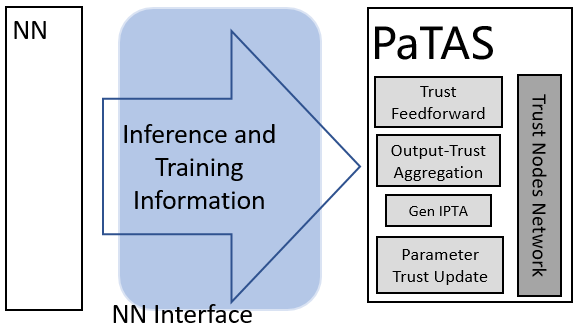
\includegraphics[width=0.5\linewidth]{img/patas/highPaTAS.png}
    \caption{High-Level Overview of the Trust Propagation in \ac{NN}}
    \label{fig:highptas}
\end{figure}

\begin{figure}
    \centering
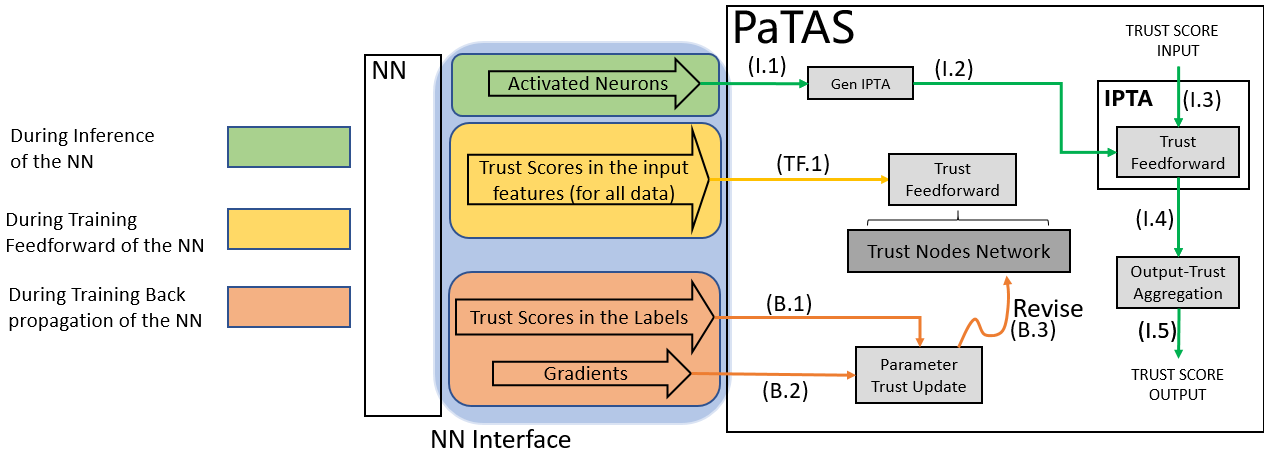
\includegraphics[width=0.8\textwidth]{img/patas/operations.png}

\caption{
    Functional flow of \ac{PaTAS-TP} integrated with a \ac{NN}, showing the interaction between the Trust Feedforward (TF), Parameter-Trust Update (B), and \ac{GenIPTA}/Output-Trust Aggregation (I) modules across the training and inference phases. \textbf{Feedforward (Training Phase):} The NN interface extracts trust scores from input features for all data being processed. These trust scores are passed to the \textit{Trust Feedforward} module (TF.1), which propagates them through the \textit{\ac{TNN}} in parallel with the \ac{NN} computations. During training, Trust Feedforward stores the trust scores of all intermediate computations in the NN, to be reused in backpropagation.    
    \textbf{Backpropagation (Training Phase):} Once the NN computes gradients, the trust scores of the labels (B.1) and the gradients (B.2) are provided to the \textit{Parameter-Trust Update}. Gradients indicate how dataset labels affect parameter updates, while label trust determines whether these updates should be considered reliable. The stored intermediate trust values are also incorporated in this process. Finally, the \textit{Parameter-Trust Update} module refines the trust values of the \ac{TNN} parameters (B.3), aligning them with the evolving learning dynamics. 
    \textbf{Inference Phase:} 
    During operation, contextual information such as the set of activated neurons is retrieved. This information is passed to \textit{\ac{GenIPTA}} (I.1), which constructs an \textit{\ac{IPTA}} corresponding to the specific inference path (I.2). The \ac{IPTA} takes input trust scores (I.3), propagates them along the path, and produces trust scores for each NN output. These can then be passed to the \textit{Output-Trust Aggregation} (I.4) which will combine them into a single consolidated trust score representing the reliability of the prediction (I.5).}
    \label{fig:ptasoperation}
\end{figure}

The backbone of \ac{PaTAS-TP} is the \emph{\acf{TNN}}, which mirrors the topology of the underlying \ac{NN} at the level of trust opinions. The \ac{TNN} is built from a single primitive: the \emph{Trust Node}, which is the trust-domain counterpart of a neuron.
\begin{definition}[Trust Node]
A \emph{Trust Node} is an abstract computational unit associated with a neuron in a \ac{NN}. It receives trust opinions on the neuron’s inputs and produces a trust opinion on the neuron’s output. The structure of a Trust Node mirrors that of its corresponding neuron, but its computation is defined over trust opinions.
\end{definition}
\noindent The parameters of the Trust Nodes are trust opinions rather than real-valued weights; they are initialized as vacuous opinions and refined during training by the Parameter-Trust Update module. The \ac{TNN} is a structured composition of Trust Nodes that mirrors the topology of the underlying \ac{NN}, propagating trust assessments layer by layer using the trust operations defined over each node. Each Trust Node receives trust opinions from its predecessors, applies its corresponding transformation, and passes the resulting opinion to its successors. 

The \ac{TNN} serves as the shared underlying representation for all four modules of \ac{PaTAS-TP}. 

\paragraph{Trust Feedforward}
The Trust Feedforward function propagates trust values through the \ac{TNN} in alignment with the \ac{NN}’s inference flow. It mirrors the layer-wise computations of the original model, but operates entirely on trust values. At each layer, trust in the inputs and parameters is combined using the trust operations, capturing how evidence flows through the network. This process produces a trust opinion for each output neuron of the \ac{NN} while also storing intermediate trust scores, which are later used by the Parameter-Trust Update.

\paragraph{Output-Trust Aggregation}
The Trust Feedforward function produces a vector of trust values, one for each output neuron. The goal of Output-Trust Aggregation is to combine these individual opinions into a single, consolidated trust score representing the overall trust in the network's output. This combination can be performed using a SL fusion operator, which fuses the trust opinions of all output Trust Nodes into one aggregated opinion. Alternatively, instead of aggregating across all outputs, one may directly consider the trust assigned to the final decision. For instance, in digit classification, if the model outputs a probability \(0.9\) for class ‘1’, the trust in the decision can be taken as the trust score associated with the output neuron for class ‘1’. More generally, the aggregation can be weighted by the strength of each output, for instance by the softmax probabilities, such that higher-confidence outputs contribute more heavily to the consolidated trust score. \DIFaddbegin \DIFadd{Finally, because every layer applies one round of discounting, aggregated trust decays geometrically with depth; a }\emph{\DIFadd{depth-normalized}} \DIFadd{variant therefore rescales the aggregated opinion by the inverse of this per-layer decay, making trust values comparable across architectures of different depths. Both the raw and the depth-normalized aggregate are used in the evaluation.
}\DIFaddend 

\paragraph{\acf{GenIPTA}}

The purpose of the \ac{GenIPTA} module is to dynamically construct a function tailored to a single, specific inference. This function, called \ac{IPTA}, reflects how trustworthy the exact computational path taken during that inference is. When an inference is performed, contextual information is recorded, such as the list of neurons activated along the path. In this case, the activation trace is used to instantiate a temporary subnetwork of Trust Nodes containing only the Trust Nodes corresponding to those activations, thereby mirroring the precise inference path of the \ac{NN}. Contextual information is not limited to activation traces. Typically, all neurons are activated to some degree, but only a subset of these activations is strongly relevant to the decision. \ac{GenIPTA} can therefore operate on truncated activation sets that retain only the most relevant neurons, which allows for more focused and interpretable trust assessments of the actual decision-making process. The \ac{GenIPTA} can also work in a more complex way by using the actual activation values of all neurons, performing a weighted trust assessment where stronger activations contribute more heavily to the trust inference.

\paragraph{Parameter-Trust Update}
The Parameter-Trust Update refines the trust opinions stored in the \ac{TNN} parameters during training, based on gradient information, input trust, and label trust to align parameter reliability with the evolving learning dynamics; its full formulation is presented in \cref{sec:param_update}.

The detailed functional flow of \ac{PaTAS-TP} across feedforward, backpropagation, and inference is illustrated in \cref{fig:ptasoperation}. 

With the architecture of \ac{PaTAS-TP} established, the following section introduces the perceptron as a minimal working example, providing concrete intuition for the operators mechanisms that underpin the Trust Feedforward computation before their generalization to deep architectures in \cref{sec:dnn_trust}.

\section{Trust Feedforward in a Simple Model: The Perceptron Case}
\label{sec:perceptron}

To illustrate the proposed trust propagation framework for the feedforward, we begin with the simple case of a single-layer perceptron. This setting provides an intuitive and tractable example that highlights the key mechanisms underlying the parallel trust function before extending them to deep \acp{NN}.

Consider a perceptron defined by a linear function:
\begin{equation}
    y' = \theta_1 s + \theta_2 \, n_r,
    \label{eq:smodel}
\end{equation}
\noindent where $s$ and $n_r$ denote input features (e.g., size and number of rooms in a apartment price estimation problem), and $\theta_1$, $\theta_2$ are the corresponding parameters.

We assume that trust assessments are available for:
\begin{itemize}
    \item the input features: $T_s$ and $T_{n_r}$,
    \item the parameters: $T_{\theta_1}$ and $T_{\theta_2}$.
\end{itemize}
\noindent The objective is to determine the resulting trust opinion $T(y')$ on the output, given these inputs.

\paragraph{Trust Propagation from Inputs}
\begin{figure}
\centering
\begin{subfigure}{0.44\linewidth}
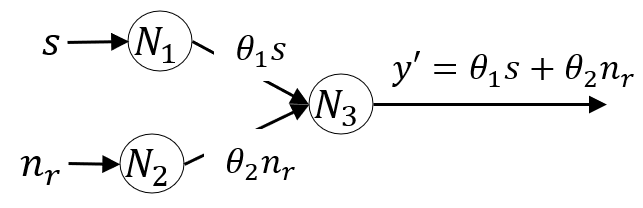
\includegraphics[width=\textwidth]{img/patas/NN1.png}
     \caption{Perceptron for \cref{eq:smodel}}
     \label{fig:nn1}
\end{subfigure}
\begin{subfigure}{0.55\linewidth}
    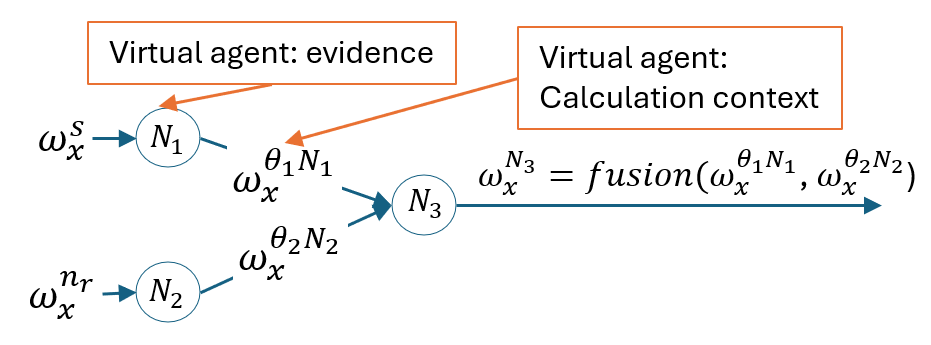
\includegraphics[width=\textwidth]{img/patas/NN1S.png}
    \caption{Parallel Trust Function for \cref{eq:smodel}}
   \label{fig:nn1s}
\end{subfigure}
\caption{Trust-propagation based solely on input-feature trust}
\label{fig:solution1}
\end{figure}

We first consider the simplified case where the parameters are assumed to be fully trusted. In this setting, the output is entirely determined by the input features, and trust propagation reduces to combining the trust opinions associated with each feature. The model specified in \cref{eq:smodel} is equivalent to the NN depicted in \cref{fig:nn1}. This network employs a linear transformation without an activation function. The input vector is:
$$ 
x = \begin{pmatrix}
    s \\
    n_r
\end{pmatrix}
$$ 
Let $\omega_x^s$ be the trust opinion on $x$ based on $s$ and  $\omega_x^{n_r}$ the trust opinion on $x$ based on $n_r$. Since the output neuron $N_3$ computes \cref{eq:smodel}, we associate this computation with two agents: $\theta_1 N_1$ from the context of computing \(\theta_1\cdot s\) and $\theta_2 N_2$ from the context of computing \(\theta_2\cdot n_r\). The trust opinion of the output neuron \(N_3\) on \(x\) is then: 
\(\omega_x^{N_3} = \mathit{fusion}(\omega_x^{\theta_1 N_1}, \omega_x^{\theta_2 N_2})\). 

The choice of the fusion operator (that we will later denote by \(\oplus\) ) depends on the semantics of \(s\) and \(n_r\) (see \cref{sec:fusion}). In this example, since $s$ and $n_r$ represent independent evidence, the fusion operator to use is cumulative fusion.

Assuming full trust in the parameters \(\theta_1\) and \(\theta_2\), we have:
\begin{align}
    \omega_x^{\theta_1 N_1} = \omega_x^{N_1} = \omega_x^{s} = T_s \, \text{ (Trust in the feature \(s\) of \(x\))} \notag \\
    \omega_x^{\theta_2 N_2} = \omega_x^{N_2} = \omega_x^{n_r} = T_{n_r} \, \text{ (Trust in the feature \(n_r\) of \(x\))} \notag 
\end{align}

Since the output value is deterministically related to the input via
\[
y' = f(x),
\]
the trust opinion of \(N_3\) on \(y'\) is the same as the trust opinion already computed for \(x\). Clearly, The transformation performed by \(f\) is encoded in the agent algebra, not in the variable algebra. Thus,
\begin{align}
    \omega_{y\prime}^{N_3} &= \omega_x^{N_3} = \omega_x^{\theta_1 N_1} \oplus \omega_x^{\theta_2 N_2} \notag \notag \\
&= \omega_x^{s} \oplus \omega_x^{n_r} = T_s \oplus T_{n_r}
\end{align}
In summary, if we define \(T_x = \begin{pmatrix}
    T_s&T_{n_r}
\end{pmatrix} \), then:
\[\pf_\Theta(T_x) = \pf_\Theta(\begin{pmatrix}
    T_s&T_{n_r}
\end{pmatrix}) =  T_s \oplus T_{n_r} \]
This formulation reflects the fact that the output trust aggregates evidence from multiple input sources, each contributing to the final prediction.

\paragraph{Incorporating Parameter Trust}
We now consider the general case where parameters are not assumed to be fully reliable. In this setting, parameter trust acts as a filtering mechanism that modulates the contribution of each input feature. Unlike the previous problem, where we fully trusted \(\theta_1\) and \(\theta_2\), here we do not fully trust these parameters, and we must account for their trust assessments. For the network to incorporate the trust in \(\theta_1\) and \(\theta_2\), we adjust the trust opinions on the features accordingly. The trust opinions are now refined.
\begin{figure}
    \centering
    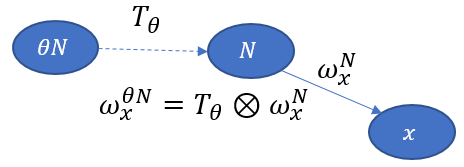
\includegraphics[width=0.4\linewidth]{img/patas/multprob2.png}
    \caption{Trust-propagation Trust Network with parameter trust\protect\footnote{The construction in our work based on the concept of Trust Node is local: it applies to a single neuron and models how the trust of one parameter modulates the trust contribution of one input. Extending this design across a path of neurons would yield a larger network whose graph structure may not satisfy the \ac{DSPG} property, as illustrated in \cref{fig:on_dspg_NN}.}.}
    \label{fig:multprob2l}
\end{figure}
As depicted in \cref{fig:multprob2l}, we model this as a small \aclu{STN}. therefore:
\begin{align}
    \omega_x^{\theta_1 N_1} = T_{\theta_1} \otimes \omega_x^{N_1} \; \text{and} \;
    \omega_x^{\theta_2 N_2} =  T_{\theta_2} \otimes \omega_x^{N_2}
\end{align}
where \(\otimes\) is a trust discounting operator. This results is consistent with the solution for problem 1 as for fully trusted \(T_\theta=(1,0,0)\), we have \(\omega_x^{\theta N} = T_{\theta} \otimes \omega_x^{N} = \omega_x^{N}\) (for any neuron \(N\)).

Finally, the resulting output trust \(\omega_{y\prime}^{N_3}\) is calculated by the fusion of these adjusted trust opinions: 
\begin{equation}
\label{eq:sol}
    \pf_\Theta(T_x) = \pf_\Theta(\begin{pmatrix}
    T_s&T_{n_r}
\end{pmatrix}) =  (T_{\theta_1}\otimes T_s)\oplus (T_{\theta_2}\otimes T_{n_r})
\end{equation}
Thus, we adjust the trust in the network output based on the trust in both the parameters and the features, ensuring that the trust propagation takes into account the trust in the parameters.

This expression highlights two key mechanisms:
\begin{itemize}
    \item \textbf{Trust Discounting:} Parameter trust modulates the reliability of each input contribution.
    \item \textbf{Trust Fusion:} The resulting contributions are aggregated to form the final output trust.
\end{itemize}
\noindent The perceptron case reveals the fundamental principles of trust propagation in \acp{NN}. First, trust is \emph{compositional}: the output trust is constructed from the contributions of individual components. Second, trust is \emph{transformed}: parameter trust acts as a filter that attenuates or amplifies the influence of input trust. Third, trust is \emph{aggregated}: multiple sources of evidence are combined using fusion operators. 

In the next section, we generalize these principles to deep \acp{NN}, where trust must be propagated across multiple layers and intermediate activations.


\section{Generalization to Deep \acp{NN}}
\label{sec:dnn_trust}

The perceptron example introduced in the previous section highlights the fundamental mechanisms of trust propagation during feedforward. We now extend these principles to deep \acp{NN}, where trust must be propagated across multiple layers and intermediate representations. Consider a \ac{NN} ($\Theta$) composed of $L$ layers, where each layer defines a transformation:
\[
h^{(l)} = f^{(l)}\left(W^{(l)} h^{(l-1)} + b^{(l)}\right), \quad l = 1, \dots, L,
\]
with $h^{(0)} = x$ and $h^{(L)} = y'$.

In the trust domain, we associate a trust opinion $T^{(l)}$ to each layer output $h^{(l)}$, such that:
\[
T^{(l)} = T\left(h^{(l)}\right), \quad l = 0, \dots, L,
\]
In particular
\[
T^{(0)} = T\left(h^{(0)}\right) = T_x, \quad T^{(L)} = T\left(h^{(L)}\right) = T(y') = Pf_\Theta(T_x)\protect
\]
Trust propagation is then defined recursively as:
\[
T^{(l)} = f_T^{(l)}\left(T^{(l-1)}, T^{(l)}_{\Theta}\right),
\]
where $T^{(l)}_{\Theta}$ denotes the trust associated with the parameters of layer $l$, and $f_T^{(l)}$ is the trust transformation corresponding to the \ac{NN} operation at that layer. This formulation extends the parallel trust function introduced in \cref{sec:trust_foundations} to a layer-wise decomposition, where trust is propagated sequentially through the network in a manner consistent with the forward computation. In practice, as developed in the \ac{GenIPTA} module, the parallel function is not defined once for the whole network but instantiated per inference, since the active computational path depends on the specific input. 

To formalize this process, we introduce the concept of trust function.
\begin{definition}[Trust Function]\label{def:trustfunc}
A \emph{Trust Function} models the transformation of trust through a Trust Node. It defines how trust opinions on the inputs of a neuron are combined to produce a trust opinion on the output. 
For a neuron that computes
\(
z^{(l)} = \sum \theta^{(l)}_i \cdot x^{(l)}_i, \quad x^{(l+1)} = \phi^{(l)}(z^{(l)}),
\)
the corresponding trust computation is given by:
\[
T_{z^{(l)}} = \bigoplus_{i=1}^{d} T_{x_{i}^{(l)}} \otimes T_{\theta_{i}^{(l)}}, \quad
T_{x^{(l+1)}} = T_{\phi^{(l)}}(T_{z^{(l)}}),
\]
\begin{itemize}
    \item \( \otimes \) is a trust discounting operator,
    \item \(\bigoplus\) is a trust fusion operator,
    \item \( T_{\phi}^{(l)} \) is the trust-equivalent of the activation function. In this work, we set it to identity function as we use ReLU as activation function.
\end{itemize}
\end{definition}

\begin{figure}[htbp]
\centering
\begin{subfigure}{0.2\textwidth}   
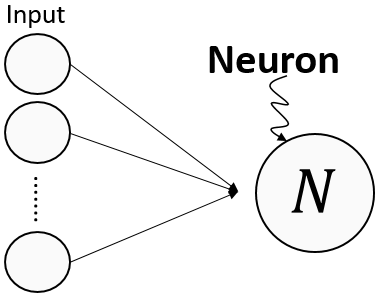
\includegraphics[width=\textwidth]{img/patas/trust_node/neuron.png}
  \caption{Structure of a Perceptron}
  \label{fig:neuron}
\end{subfigure}
\begin{subfigure}{0.2\textwidth}
  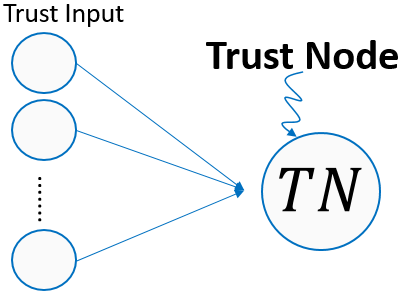
\includegraphics[width=\textwidth]{img/patas/trust_node/trustnode.png}
  \caption{Mirrored Trust Structure}
  \label{fig:tns}
\end{subfigure}

\begin{subfigure}{0.45\textwidth}
  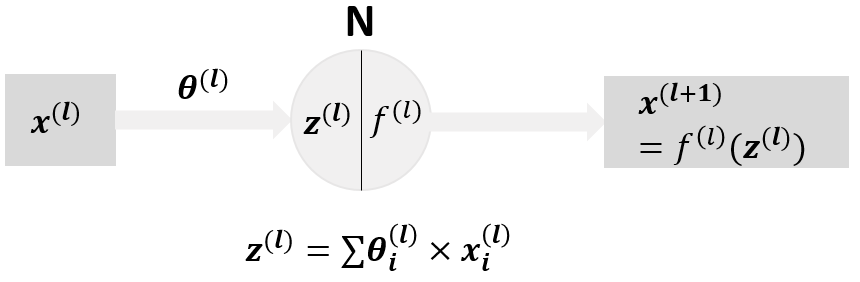
\includegraphics[width=\textwidth]{img/patas/trust_node/neurop.png}
  \caption{Perceptron Operation}
  \label{fig:neuronfunc}
\end{subfigure}
\begin{subfigure}{0.45\textwidth}
  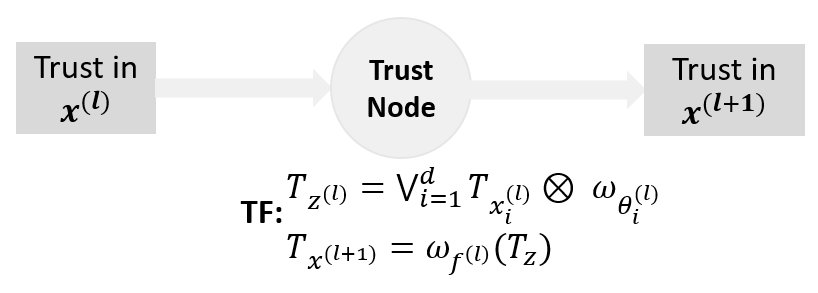
\includegraphics[width=\textwidth]{img/patas/trust_node/tnop.png}
  \caption{Trust Function Operation}
  \label{fig:tnf}
\end{subfigure}

\caption{Illustration of the Trust Node structure and computation}
\label{fig:trustnode}
\end{figure}

% In particular, the two fundamental operations identified in the perceptron case generalize as follows:
% \begin{itemize}
%     \item \textbf{Weighted Contributions (Discounting):} The influence of an input activation on a neuron is modulated by the trust in the corresponding weight. This is modeled using the trust discounting operator:
%     \[
%     T_{\text{contrib}} = T_{\theta} \otimes T_{\text{input}}.
%     \]

%     \item \textbf{Aggregation (Fusion):} Multiple contributions to a neuron are combined using a fusion operator:
%     \[
%     T_{\text{node}} = \bigoplus_i T_{\text{contrib}, i}.
%     \]
% \end{itemize}
% Activation functions can be interpreted as transformations that preserve or reshape trust without introducing new sources of evidence. In this work, we assume that activation functions do not alter the trust opinion directly, but only affect the structure of the propagation by activating or deactivating certain paths.

\Cref{fig:trustnode} illustrates the structural correspondence between a standard neuron and its associated Trust Node. \cref{fig:neuron,fig:tns} show how the mirrored trust structure is derived from the original perceptron, while \cref{fig:neuronfunc,fig:tnf} contrast the numerical computation of the neuron with the trust-domain computation of the Trust Function, in which multiplication is replaced by discounting and summation by fusion. 

% Combining these elements, trust propagation in a deep \ac{NN} proceeds as follows:
% \begin{enumerate}
%     \item \textbf{Initialization:} Assign trust opinions $T^{(0)} = T(x)$ to the input features.

%     \item \textbf{Layer-wise Propagation:} For each layer $l = 1, \dots, L$:
%     \begin{itemize}
%         \item Compute discounted contributions from the previous layer using parameter trust.
%         \item Aggregate contributions using a fusion operator.
%         \item Assign the resulting trust to the current layer: $T^{(l)}$.
%     \end{itemize}

%     \item \textbf{Output Trust:} The final trust opinion is given by $T(y') = T^{(L)}$.
% \end{enumerate}

\begin{algorithm}
\caption{Trust Feedforward}
\begin{algorithmic}[1]
\Require Input trust $T^{(0)} = T(x)$, parameter trust 
         $\{T^{(l)}_\Theta\}_{l=1}^{L}$
\Ensure Output trust $T(y') = T^{(L)}$

\For{each layer $l = 1, \dots, L$}
    \For{each neuron $i$ in layer $l$}
        \State Compute discounted contributions:
        \[
        T_{\text{contrib},j} = T_{\theta^{(l)}_{i,j}} \otimes T^{(l-1)}_{x_j}, 
        \quad \forall j \in \mathcal{N}(i)
        \]

        \State Aggregate contributions via fusion:
        \[
        T_{z^{(l)}_i} = \bigoplus_{j \in \mathcal{N}(i)} T_{\text{contrib},j}
        \]
        \State Apply activation trust:
        \[
        T^{(l)}_{x_i} = T_{\phi^{(l)}}(T_{z^{(l)}_i})
        \]
    \EndFor
\EndFor
\State \Return $T(y') = T^{(L)}$
\end{algorithmic}
\label{alg:trustff}
\end{algorithm}

\DIFaddbegin \subsection{\DIFadd{Extension to Convolutional Architectures}}
\label{sec:conv_trust}
\DIFadd{The construction above is stated for fully connected layers, but nothing in it is specific to them; what changes in a }\ac{CNN} \DIFadd{is weight sharing. }\ac{PaTAS-TP} \DIFadd{mirrors a convolutional layer with $c_{\mathrm{in}}$ input channels, $c_{\mathrm{out}}$ output channels, and kernel size $k$ by one opinion matrix of shape $(c_{\mathrm{in}} k^2 + 1) \times c_{\mathrm{out}}$, exactly the flattened kernel matrix that also carries the layer's gradients, so the Parameter-Trust Update of }\cref{sec:param_update} \DIFadd{applies unchanged. For the feedforward, the input pixel opinions are fused into per-channel opinions and the layer is applied as the standard dense discount-fusion rule on the flattened kernel matrix; this }\emph{\DIFadd{uniform-trust reduction}} \DIFadd{is exact whenever the input trust is spatially uniform (the trusted, vacuous, and distrusted profiles used throughout) and an approximation otherwise. ReLU and pooling remain identity in opinion space, and a residual skip connection is mapped to averaging fusion of the block's input and output opinions.
}

\DIFadd{The }\ac{IPTA} \DIFadd{generalizes as well, with one conceptual change. In a fully connected network an inference path selects }\emph{\DIFadd{weights}}\DIFadd{: inactive neurons remove their rows from the trust computation. Under weight sharing a path cannot select weights, only }\emph{\DIFadd{applications}} \DIFadd{of a filter, since the same kernel is applied at every spatial position. The convolutional }\ac{IPTA} \DIFadd{therefore weights each channel's contribution by its }\emph{\DIFadd{participation degree}}\DIFadd{: the fraction of spatial positions at which the channel's post-ReLU output is positive for the given input. Formally, the discount-fusion step becomes a weighted fusion in which row $j$ of the opinion matrix enters with weight $w_j$ equal to the producing channel's participation (bias rows keep weight $1$). For binary participation this reduces }\emph{\DIFadd{exactly}} \DIFadd{to the row-pruned computation of the fully connected }\ac{IPTA}\DIFadd{, so the convolutional variant is a strict generalization: channels the forward pass never activated contribute nothing, and partially active channels contribute in proportion to their actual involvement in the decision.
}

\DIFaddend \Cref{alg:trustff} formalizes this layer-wise computation as the complete Trust Feedforward pipeline. This generalization demonstrates that trust propagation can be integrated into deep \acp{NN} without altering their structure, by defining a parallel computation over trust opinions. It makes the link between output trust $T_{y'}$, input trust $T_{x}$, and parameter trust $T_{\theta}$: 
\[T_{x} \xrightarrow{T_\theta} T_{y'}.\] In the next section, we focus on how parameter trust is computed during training, completing the link between dataset trust and model trustworthiness:
\[T_{\dataset} \rightarrow T_\theta.\] 

\section{Parameter-Trust Update}\label{sec:param_update}
The Parameter-Trust Update is the mechanism through which \ac{PaTAS-TP} adapts the trust associated with model parameters during training. Its objective is to ensure that parameter trust reflects both the observed behavior of the model and the reliability of the training data. Its design is inspired by the standard backpropagation algorithm used in \ac{NN} training, where gradients quantify how much each parameter contributes to the output error. By leveraging these gradients as evidence, \ac{PaTAS-TP} updates parameter trust in a way that mirrors the learning dynamics of the underlying model.

To ground the design, we briefly recall the standard parameter update in \ac{NN} training. For a parameter $\theta$, gradient descent updates are given by:
\begin{equation}
\label{eq:gd1}
\theta \leftarrow \theta - l_r  \frac{\partial \mathcal{L}}{\partial \theta},
\end{equation}
where $l_r$ is the learning rate, $\mathcal{L}$ is the loss function, and $\frac{\partial \mathcal{L}}{\partial \theta}$ is the gradient. These gradients are computed recursively using the chain rule:
\begin{equation}
\label{eq:gd2}
\frac{\partial \mathcal{L}}{\partial \theta^{(l)}_{i,j}}
= \delta^{(l)}_i x^{(l-1)}_j,
\end{equation}
where $\theta^{(l)}_{i,j}$ denotes the weight connecting neuron $j$ in layer $(l-1)$ to neuron $i$ in layer $l$, $\delta^{(l)}_i$ is the error term of neuron $i$, and $x^{(l-1)}_j$ is the activation from the previous layer.

In particular, \cref{eq:gd2} shows that gradients factor into an error term and an input activation, revealing that parameter updates depend jointly on gradient signals, input activations, and learning dynamics. \ac{PaTAS-TP} mirrors this structure by incorporating gradient information, input trust, and label trust as analogous sources of evidence in the Parameter-Trust Update. At a high level, the parameter-trust update process combines three sources of information: (i) gradient-based evidence derived from backpropagation, (ii) trust in the labels within the current training batch, and (iii) trust in the input features and intermediate computations recorded during feedforward. These elements are integrated to revise and refine the trust assigned to each parameter. The notation used throughout this subsection is summarized in \cref{tab:symbols}, and the complete update procedure is given in \cref{alg:trustupdate}.

\begin{algorithm}
\caption{Parameter-Trust Update Algorithm}
\begin{algorithmic}[1]

    \Function{ParameterTrustUpdate}{$g, T_y, \epsilon$}
        \State \textbf{Summary:} Revises and updates the trust parameters of the Trust Nodes by combining gradient evidence, label trust, and neuron input trust, under mini-batch training.

        \State \textbf{Step 1:} Compute the aggregated trust in the labels
        \State $T_{y_\text{batch}}  \longleftarrow  \bigwedge_{y \in y_\text{batch}} T_y$

        \For{each layer $l$}
            \For{each neuron $n_i^{(l)}$}
                \State \textbf{Step 2:} Gather gradient $g$ for neuron $n_i^{(l)}$
                \State $g^{(l)}_i  \longleftarrow  \{\, g^{(l)}_{i,j} \;|\; j \in \mathcal{N}(i)\,\}$

                \State \textbf{Step 3:} Compute trust for neuron $n_i^{(l)}$
                \State $T_{n_i \mid y_\text{batch}}  \longleftarrow $ \Call{NodeTrust}{$g^{(l)}_i, T_{y_\text{batch}}, \epsilon$}

                \State \textbf{Step 4:} Deduce overall trust in neuron $n_i^{(l)}$ 
                \State $T_{n_i \parallel Y_\text{batch}}  \longleftarrow $ \Call{DeduceTrust}{$T_{n_i \mid y_\text{batch}}, T_{n_i \mid \overline{y_\text{batch}}}, T_{y_\text{batch}}$}

                \For{each incoming edge $j$ to $n_i^{(l)}$}
                    \State \textbf{Step 5:} Revise parameter trust with node trust
                    \State $T_{\theta_{i,j}^{(l)}}  \longleftarrow $ \Call{Revise}{$T_{\theta_{i,j}^{(l)}}, T_{n_i \parallel Y_\text{batch}}$}

                    \State \textbf{Step 6:} Update parameter trust with auxiliary factors
                    \State $T_{\theta_{i,j}^{(l)}} \longleftarrow $ \Call{Update}{$T_{\theta_{i,j}^{(l)}}, T_{x^{(l-1)}_j}, T_{y_\text{batch}}$}
                \EndFor
            \EndFor
        \EndFor
    \EndFunction

    \Function{NodeTrust}{$g^{(l)}_i, T_{y_\text{batch}}, \epsilon$}
        \State Count $r$: \#edges with $|g^{(l)}_{i,j}| < \epsilon$ 
        \State Count $s$: \#edges with $|g^{(l)}_{i,j}| \geq \epsilon$ 
        \State Map $(r,s)$ into a binomial opinion using Baseline-Prior Quantification
        \State \Return $T_{n_i \mid y_\text{batch}}$
    \EndFunction

    \Function{DeduceTrust}{$T_{n_i \mid y_\text{batch}}, T_{n_i \mid \overline{y_\text{batch}}}, T_{y_\text{batch}}$}
        \State $T_{n_i \mid \overline{y_\text{batch}}}  \longleftarrow  (0,0,1)$
        \State \Return $T_{n_i \parallel Y_\text{batch}} = T_{y_\text{batch}} \circledcirc (T_{n_i \mid y_\text{batch}}, T_{n_i \mid \overline{y_\text{batch}}})$
    \EndFunction

    \Function{Revise}{$T_{\theta_{i,j}^{(l)}}, T_{n_i \parallel Y_\text{batch}}$}
        \State \Return $T_{\theta_{i,j}^{(l)}} \circleddash T_{n_i \parallel Y_\text{batch}}$
    \EndFunction

\end{algorithmic}
\label{alg:trustupdate}
\end{algorithm}
The procedure described in \cref{alg:trustupdate} operates at the level of mini-batches and iterates over all layers and neurons of the network. For each neuron, it first derives a trust assessment based on gradient evidence and the reliability of the training labels, and then propagates this information to update the trust associated with its incoming parameters. More specifically, the update process can be decomposed into three main stages: (i) aggregation of label trust at the batch level, (ii) estimation of neuron-level trust using gradient information, and (iii) revision and adjustment of parameter trust using both inferred neuron trust and auxiliary factors such as input trust. We now describe these steps in detail.

The algorithm runs once per batch and begins by computing a combined trust opinion over all labels in the current batch (Line 3):
\(
T_{y_\text{batch}} = \bigwedge_{y \in y_\text{batch}} T_y
\).

This combined opinion serves as a foundation for conditioning the trust in each parameter.

For each neuron \(n_i^{(l)}\) at index \(i\) in layer \(l\), we compute:
\begin{itemize}
    \item \( T_{n_{i}^{(l)} \mid y_\text{batch}} \) (Line 9), the trust conditioned on the current batch labels. This is inferred by checking each incoming weight gradient \( g^{(l)}_{i,j} \): if \( |g^{(l)}_{i,j}| < \epsilon\)\footnote{The threshold $\epsilon$ is not a tuned hyperparameter but a sensitivity parameter used only in the \textsc{NodeTrust} function to distinguish weak from strong gradients. Its value can be chosen in different reasonable ways depending on the desired sensitivity.}
 it is counted as positive evidence \( r \), otherwise as negative evidence \( s \). These counts are then mapped into a binomial opinion using the Baseline-Prior Quantification model.
    \item \( T_{n_{i}^{(l)} \mid \overline{y_\text{batch}}} \), the trust when the true batch labels are not \( y_\text{batch} \). Since no concrete evidence is available for this case, it is initialized to a vacuous opinion: \( (0, 0, 1) \).
    \item A deduced trust \( T_{n_{i}^{(l)} \parallel Y_\text{batch}} \) (Line 11) using the inferential deduction operator \( \circledcirc \), combining the two conditional opinions with \( T_{y_\text{batch}} \).
\end{itemize}

Then for each incoming edge \( j\) of neuron \( i \), the parameter trust \( T_{\theta_{i,j}^{(l)}} \) is updated in two stages:
\begin{enumerate}
    \item Revision with deduced trust using fusion (Line 14):
    \[
    T_{\theta_{i,j}^{(l)}} \leftarrow T_{\theta_{i,j}^{(l)}} \circleddash T_{n_{i}^{(l)} \parallel Y_\text{batch}}
    \]
    \item Adjustment with auxiliary factors (Line 16):
    During training, the update of parameter $\theta_{i,j}^{(l)}$ depends not only on its current value but also on auxiliary factors such as the input $x^{(l-1)}_{j}$, and the label $y_\text{batch}$ (see \cref{eq:gd1,eq:gd2}).  
To reflect this, we adjust parameter trust using:
\[
    T_{\theta_{i,j}^{(l)}} \longleftarrow T_{\theta_{i,j}^{(l)}} \odot (T_{x_j^{(l-1)}} \oslash T_{y_\text{batch}}).
\]
Here, $\odot$ is the binomial multiplication operator and $\oslash$ is defined as:
\begin{align}
    (b,d,u) &= (b_1, d_1, u_1) \oslash (b_2, d_2, u_2), \\
    b &= \min(b_1, b_2), \notag \\
    d &= \max(d_1, d_2), \notag \\
    u &= 1 - (b+d). \notag
\end{align}
This formulation reflects the fact that both unreliable features and mislabeled data can strongly bias parameter updates. The use of min and max provides a conservative aggregation: trust cannot exceed the weakest evidence, and distrust must reflect the strongest warning. It ensures that trust in both input features and labels is explicitly propagated into the parameter trust.
\end{enumerate}

\DIFaddbegin \paragraph*{\DIFadd{Scale-Tied Threshold.}}
\DIFadd{The threshold $\epsilon$ used by }\textsc{\DIFadd{NodeTrust}} \DIFadd{separates weak from strong gradients, and its natural scale is that of the gradients themselves, which varies across tasks and across layers. Rather than treating $\epsilon$ as an absolute constant, we therefore also define a }\emph{\DIFadd{scale-tied}} \DIFadd{variant: for each layer, $\epsilon_{\mathrm{layer}} = c \cdot \mathrm{median}(|\delta|)$, where the median gradient magnitude is estimated over the first revision batches of that layer and then frozen, and $c$ is a single dimensionless constant ($c = 0.5$ unless stated otherwise). This makes the stability criterion relative to the task's own gradient scale: the same rule instantiates thresholds differing by nearly two orders of magnitude across the tasks studied here without any per-task tuning. Its empirical validation is reported in }\cref{sec:patas-discussion}\DIFadd{.
}


\DIFaddend \paragraph*{Computational Overhead during \ac{NN} training.}
The proposed \ac{PaTAS-TP} operates in parallel with the primary \ac{NN} and mirrors its computational flow using subjective opinions. As a result, the overall execution time cost can be roughly expressed as:
\[
\mathcal{C}_{\text{with \ac{PaTAS-TP}}} \approx \mathcal{C}_{\text{comm}} + \max(\mathcal{C}_{\text{PaTAS-TP}}, \mathcal{C}_{\text{NN}}),
\]
where \(\mathcal{C}_{\text{comm}}\) denotes the communication overhead between the \ac{NN} and the \ac{PaTAS-TP}. Each \ac{PaTAS-TP} operation is performed over subjective opinions represented by \DIFdelbegin \DIFdel{multiple }\DIFdelend \DIFaddbegin \DIFadd{three stored }\DIFaddend components (trust, distrust, uncertainty\DIFdelbegin \DIFdel{, and a fixed base rate ), leading to a higher computational cost compared to standard scalar operations. In practice, this results in \(\mathcal{C}_{\text{PaTAS-TP}} \approx 4 \times \mathcal{C}_{\text{NN}}\). Consequently, the overall runtime is }\DIFdelend \DIFaddbegin \DIFadd{; the base rate is a shared constant), giving an analytical estimate of roughly \(\mathcal{C}_{\text{PaTAS-TP}} \approx 3 \times \mathcal{C}_{\text{NN}}\) for the propagation arithmetic and a threefold memory overhead for the opinion parameters. Measured costs on an A100 GPU (784-512-10 architecture) are consistent with this estimate at inference time: trust propagation costs $0.43$\,ms per batch, amortizing from $14.8\times$ overhead at batch size 1 to $3.7\times$ at batch size 512. During training, wall-clock time is instead }\DIFaddend dominated by the \DIFaddbegin \DIFadd{synchronous gradient stream and revision when }\DIFaddend \ac{PaTAS-TP} \DIFdelbegin \DIFdel{computation, yielding the approximation:
}\[
\DIFdel{\mathcal{C}_{\text{with \ac{PaTAS-TP}}} \approx \mathcal{C}_{\text{comm}} + 4\mathcal{C}_{\text{NN}}.
}\]%DIFAUXCMD
\DIFdel{Despite this overhead, the parallel design }\DIFdelend \DIFaddbegin \DIFadd{is attached in-process (roughly $7$ versus $2200$ optimization steps per second unattached), an engineering bottleneck of the socket-based prototype rather than of the method; since training requires no value from }\ac{PaTAS-TP}\DIFadd{, the revision can equally run as an offline replay of the recorded gradient stream after training, which is how all cached experiments in this chapter were produced. The parallel design thus }\DIFaddend ensures that trust propagation does not interfere with the execution of the primary model, making the approach suitable for \DIFdelbegin \DIFdel{real-time }\DIFdelend monitoring scenarios where interpretability and reliability are critical.
\DIFdelbegin \DIFdel{Moreover since the training does not need any value from }%DIFDELCMD < \ac{PaTAS-TP}%%%
\DIFdel{, it can still continue while }%DIFDELCMD < \ac{PaTAS-TP} %%%
\DIFdel{takes the time needed to complete its operations.
}\DIFdelend 



\section{Theoretical Properties of \ac{PaTAS-TP}}\label{sec:ptastheory}
To ensure that \ac{PaTAS-TP} provides reliable and interpretable trust assessments, we first establish several fundamental theoretical properties describing its stability and consistency.
\subsection{Convergence of \ac{PaTAS-TP}}
\label{sec:ptas_convergence}

The convergence of the \ac{PaTAS-TP} is governed by the stability of its inputs and the structure of its recursive Parameter-Trust Update process. During training, \ac{PaTAS-TP} updates the internal trust opinions associated with network parameters using trust opinions on the inputs, labels, hyperparameters, and gradient information. This update mechanism is outlined in \cref{alg:trustupdate}. 
\begin{theorem}[Convergence of \ac{PaTAS-TP} Creation\footnote{All proofs of the theorems in this section are provided in the \appp (\cref{app:proof}).}]\label{thm:convergence}
Let a \ac{NN} be trained until convergence, and let its associated \ac{PaTAS-TP} operate with:
\begin{itemize}
    \item a stable input trust assessment $T_x$,
    \item a stable label trust assessment $T_y$,
    % \item a stable hyperparameter trust $T_{lr}$,
    % \item and converging back propagation gradients $g$.
\end{itemize}

Let $T_\theta^{(n)}$ denote the trust opinion at iteration $n$ for parameter $\theta$. If the revision of the trust in the weights is performed as specified in \cref{alg:trustupdate}, then the \ac{PaTAS-TP} parameter will converge. Specifically, if the revision operator $\circleddash$ is a fusion operator, the sequence converges to the update opinion $q$ (or remains at $\omega_0$ if $q$ is vacuous, as established in \cref{thm:arithm}); if $\circleddash$ is the binomial multiplication operator $\odot$, the sequence converges componentwise, with disbelief accumulating toward $1$ when $d_q > 0$ and belief decaying toward $0$ when the projected probability $p_q < 1$, as established in \cref{thm:geo}.
\end{theorem}


\subsection{Symmetry and Invariance Properties of \ac{PaTAS-TP}}\label{sec:ptassyminv}

\begin{theorem}[\ac{PaTAS-TP} Inference on Vacuous Input Yields Vacuous Output]\label{thm:infvac}
Let \( \omega^\emptyset = (0, 0, 1, a) \) denote a vacuous binomial opinion over any variable, with arbitrary base rate \( a \in [0, 1] \). Then the following two properties hold:

\begin{enumerate}
    \item \emph{Vacuous discounting: The discounting of a vacuous opinion is vacuous.} \\
    For any trust value binomial opinion \(\omega^A_B \), the discounted opinion
    \(
    \omega^{[A;B]}_X = \omega^A_B \otimes (0,0,1,a)= (0,0,1,a)
    \)
    \item \emph{Vacuous Feedforward: \ac{PaTAS-TP} Feedforward on a Vacuous Input is Vacuous.} \\
     Let \( T_x = (0,0,1,a)\) be the trust assessment of an input to \ac{PaTAS-TP}. Then for any parameter trust configuration \( T_\theta \), the output trust assessment satisfies:
    \(
    T_y = \text{IPTA}(T_x) = (0,0,1,a).
    \)
\end{enumerate}
\end{theorem}
\begin{definition}[Symmetric Binomial Opinions]
Let \(\omega=(b, d, u, a)\) be a binomial opinion. The opinion $\bar{\omega} = (d, b, u, a)$ is called the \emph{symmetric} of $\omega$. 
\end{definition}
\begin{theorem}[Symmetric Inference under \ac{PaTAS-TP}]\label{thm:sym}
Let $T_\theta$ be a \ac{PaTAS-TP} feedforward function, and let $x = (b, d, u, a)$ be any binomial opinion with symmetric counterpart $\bar{x} = (d, b, u, a)$. Then the outputs $y = T_\theta(x)$ and $\bar{y} = T_\theta(\bar{x})$ are also symmetric, i.e.,
\(
y = (b', d', u', a), \quad \bar{y} = (d', b', u', a).
\)

In particular, the uncertainty is preserved:
\(
u_y = u_{\bar{y}},
\)
and the belief in one output equals the disbelief in the other:
\(
b_y = d_{\bar{y}}, \quad d_y = b_{\bar{y}}.
\)
\end{theorem}
\begin{remark}
For a fully trusted input $x = (1,0,0)$, the discounting operator yields $\omega_\theta \otimes x = (P, 0, 1-P)$, which has zero disbelief. Since fusion preserves zero disbelief across inputs, the output satisfies $d_y = 0$. By the same argument applied to $\bar{x} = (0,1,0)$, which produces zero belief after discounting, the output satisfies $b_{\bar{y}} = 0$. 

In other words, a fully trusted input $x = (1,0,0)$ yields an output with $d_y = 0$, and a fully distrusted input $\bar{x} = (0,1,0)$ yields an output with $b_{\bar{y}} = 0$. 

This property illustrates a directional preservation of evidence: a fully trusted input cannot produce a non-zero disbelief mass at the output, regardless of the trustworthiness of the parameters. Symmetrically, a fully distrusted input cannot produce a non-zero belief mass at the output. Non-zero disbelief in the output can arise only from disbelief already present in the input; it is never introduced by the \ac{PaTAS-TP}.
\end{remark}

These properties serve as fundamental consistency checks, ensuring predictable behavior under neutral, vacuous, or balanced evidence.


\DIFaddbegin \section{\DIFadd{Per-Sample Trust at Inference: Input Conformity and Composed Scores}}
\label{sec:inference-trust}

\DIFadd{The propagation machinery of the preceding sections consumes an input-trust opinion $T_x$ but does not prescribe where it comes from. In the controlled experiments of }\cref{sec:patas-tp-evaluation}\DIFadd{, $T_x$ is supplied externally as a scenario assumption (fully trusted, vacuous, or distrusted). For deployment, however, an externally supplied opinion is rarely available per input, and using a constant fully trusted opinion would make the propagated score carry no per-sample input information at all. This section instantiates the estimation-from-data route: input opinions are derived from each sample's conformity to the training-data statistics, then composed with the path trust into a single per-sample score.
}

\subsection{\DIFadd{Conformity-Based Input Opinions}}
\label{sec:conformity}
\DIFadd{Let the clean training features be $x^{(1)},\dots,x^{(n)} \in \mathbb{R}^m$, with marginal mean $\mu_j$ and standard deviation $\sigma_j$ per feature $j$, and let $S$ be a robust span of the feature matrix (the difference between its $99.5$th and $0.5$th percentiles). The }\emph{\DIFadd{effective deviation}} \DIFadd{floors each $\sigma_j$ at a fraction of the span, $\sigma^{\mathrm{eff}}_j = \max(\sigma_j, 0.02\, S)$, so that near-constant features cannot produce unbounded standardized deviations from minimal perturbations. For an input $x$, the standardized deviation is $z_j = |x_j - \mu_j| / \sigma^{\mathrm{eff}}_j$ and the conformity is
}\[
\DIFadd{g_j = \exp\!\big(-\tfrac{1}{2}\max(z_j - 1, 0)^2\big) \in (0,1}]\DIFadd{,
}\]
\DIFadd{so deviations within one effective standard deviation are fully conforming and only the excess erodes conformity. Each feature further receives a }\emph{\DIFadd{reliability weight}} \DIFadd{$w_j = \min\big((\sigma_{\mathrm{ref}} / \sigma^{\mathrm{eff}}_j)^2, 64\big)$ with $\sigma_{\mathrm{ref}}$ the median effective deviation: a feature with a tight training distribution is a reliable witness whose violation is unambiguous, while the cap bounds the influence any single feature can exert. Feature $j$ contributes evidence $r_j = N w_j g_j$ and $s_j = N w_j (1-g_j)$ with base evidence mass $N = 50$, mapped to a binomial opinion by the same Baseline-Prior Quantification used for parameter trust (prior weight $W = 2$, }\cref{chap:dataset-trust}\DIFadd{). The pooled per-sample input trust $P_{\mathrm{input}}$ is the projected probability of the opinion obtained from the summed evidence $(\sum_j r_j, \sum_j s_j)$, corresponding to cumulative fusion of independent evidence sources. All constants are fixed once and shared by every dataset in the evaluation.
}

\paragraph*{\DIFadd{Applicability Diagnostics.}}
\DIFadd{The construction is a per-feature marginal model, and its informativeness can be predicted }\emph{\DIFadd{before any model is trained}} \DIFadd{from the weight statistics it induces on the clean training features. Registered domains, where semantic content sits at fixed positions (centered digits, garment silhouettes), concentrate weight mass in tight, reliable witness features; unregistered natural imagery has no such witnesses, and the diagnostics predict that marginal conformity will be uninformative there. This prediction is borne out empirically in Experiment~4 (}\cref{tab:diss-diagnostics}\DIFadd{): the datasets with concentrated witnesses are exactly those where conformity detects corruption, and the boundary case flagged by the diagnostics is exactly where it fails. The diagnostics therefore serve as an a-priori deployment gate for the input-side signal.
}

\subsection{\DIFadd{Composed Per-Sample Score}}
\label{sec:composed}
\DIFadd{At inference, three trust quantities are available for a sample $x$: the input conformity trust $P_{\mathrm{input}}(x)$; the }\emph{\DIFadd{path trust}} \DIFadd{$P_{\mathrm{model}}(x)$, the projected probability of the predicted class's opinion obtained by feedforwarding a fully trusted input through the }\ac{IPTA} \DIFadd{instantiated from $x$'s activation path, which isolates the reliability of the parameters actually used; and the model's own confidence $\hat{p}(x)$, its maximum softmax probability. The composed trust factor is the serial discount
}\[
\DIFadd{P(x) = P_{\mathrm{model}}(x) \cdot P_{\mathrm{input}}(x),
}\]
\DIFadd{the }\ac{SL} \DIFadd{projected probability of trusting the prediction through both the path and the input source. For selective prediction the trust factor is combined with confidence through class-prior anchoring,
}\[
\DIFadd{s(x) = P(x)\, \hat{p}(x) + \big(1 - P(x)\big)/K,
}\]
\DIFadd{with $K$ the number of classes: when trust is full the score is the model's confidence, and as trust vanishes the score falls to the uninformed prior $1/K$ rather than to an arbitrary zero. An alternative, fully propagated variant pushes the per-feature opinions through the }\ac{IPTA} \DIFadd{feedforward instead of composing at the output; the averaging fusion inside the opinion product compresses the per-sample input signal, so serial composition is used as the default and the propagated variant is kept as an ablation.
}

\paragraph*{\DIFadd{Deployment Semantics.}}
\DIFadd{The composed score is a trust-weighted confidence, not a replacement for confidence. Confidence ranks correctness }\emph{\DIFadd{within}} \DIFadd{the training distribution; trust flags inputs and parameters that }\emph{\DIFadd{leave}} \DIFadd{it. The operational reading is therefore two-stage: gate on the trust factor (and on the applicability diagnostics), then rank by confidence among trusted inputs. The evaluation below makes this division of labor explicit and quantifies each factor's contribution separately.
}

\DIFaddend \section{Evaluation and Results}\label{sec:patas-tp-evaluation}

The goal of our evaluation is to validate the \ac{PaTAS-TP} both theoretically and empirically. Specifically, we aim to demonstrate that \ac{PaTAS-TP} produces interpretable trust estimates that (i) converge during training under specific conditions, (ii) respect symmetry and invariance properties, and (iii) are able to provide interpretable assessments under realistic conditions such as noisy features, corrupted labels, or adversarial perturbations\DIFaddbegin \DIFadd{, and (iv) provide per-sample and model-level signals whose value against established uncertainty-quantification and detection baselines can be attributed to identifiable mechanisms}\DIFaddend .  

Our evaluation approach combines controlled synthetic degradations with real-world datasets. We vary the trustworthiness of inputs ranging from fully trusted, fully uncertain, to fully distrusted, and observe how the created \ac{PaTAS-TP} propagates these trust assessments through the network. For each scenario, we track three complementary metrics: trust mass (belief), uncertainty mass, and distrust mass (disbelief) of the trust opinion output by \ac{PaTAS-TP}. We also compare these values against standard model accuracy (after training) to understand how input trust affects output reliability. We conduct \DIFdelbegin \DIFdel{three }\DIFdelend \DIFaddbegin \DIFadd{four }\DIFaddend experiments of increasing complexity\DIFdelbegin \DIFdel{based on three different datasets}\DIFdelend :  
\begin{enumerate}
  \item \emph{Breast Cancer Classification}, to assess behavior on a small, tabular medical dataset.  
  \item \emph{MNIST Digit Classification}, to evaluate \ac{PaTAS-TP} across multiple \ac{NN} architectures under uncertainty.
  % and randomized trust assignments.  
  \item \emph{Poisoned MNIST}, to evaluate \ac{PaTAS-TP} and \ac{IPTA} in the presence of adversarial corruption and data poisoning.  
  \DIFaddbegin \item \emph{\DIFadd{Comparative Trust Evaluation}}\DIFadd{, to evaluate the composed per-sample score of }\cref{sec:inference-trust} \DIFadd{against established uncertainty and detection baselines on }\ac{OOD} \DIFadd{and corruption detection, on fully connected and convolutional architectures, together with a test-data-free training-quality audit.
}\DIFaddend \end{enumerate}


\subsection{Experimental Setup }
\subsubsection{Experiment 1 - Breast Cancer Classification}\label{exp:1}
We use the \href{https://archive.ics.uci.edu/dataset/17/breast+cancer+wisconsin+diagnostic}{Breast Cancer Wisconsin (Diagnostic) Dataset}~\cite{breastcancer-wisconsin}, containing 569 samples with 30 numeric features (e.g., radius, area, symmetry) derived from breast mass fine needle aspirates. The \ac{NN} classifies the tumors into benign or malignant categories.
The \ac{NN} architecture consists of 30 input neurons, 16 hidden neurons, and 2 output neurons, with ReLU activation in the hidden layer and Softmax in the output. The model is trained for 15 epochs with a batch size of 64 and a learning rate of 0.2, achieving 98\% accuracy when the data are not modified.

For the evaluation, we degrade the training data in controlled ways and assign corresponding Subjective Logic trust assessments. We consider three extreme trust profiles (fully trusted \((1,0,0)\), fully distrusted \((0,1,0)\), and fully uncertain \((0,0,1)\)) for both input features and label. These are combined (for inputs and label assessment) to form nine combinations. These dogmatic and vacuous opinions serve as canonical boundary cases in Subjective Logic: they express maximal trust, maximal distrust, and maximal uncertainty, respectively. We additionally include two intermediate scenarios, introduced below, to illustrate how \ac{PaTAS-TP} behaves under partial trust and partial distrust.

In practice, feature and label trust degradation may arise from poor-quality imaging, human annotation errors, or flaws in the preprocessing pipeline. In this experiment and the following ones, we simulate degradations using controlled perturbation functions. For fully uncertain feature opinion, we introduce additive uniform noise 

\[
x' = x + \mu, \quad \mu \sim U(-\eta, \eta),
\]
where 
\(
\eta = 0.3 \times \max(\text{features}).
\)
Each feature is perturbed with probability $0.3$. 
After noise addition, if $x'$ lies outside the valid range 
$[\min(\text{features}), \max(\text{features})]$, it is clipped to the corresponding boundary:
\[
x' = 
\begin{cases}
\min(\text{features}), & x' < \min(\text{features}), \\
\max(\text{features}), & x' > \max(\text{features}), \\
x', & \text{otherwise}.
\end{cases}
\]
To model distrust, we generate corrupted inputs by sampling from a uniform distribution over the feature space:
\[
x' \sim U\left(\min\left(\text{features}\right), \max\left(\text{features}\right)\right),
\]

\noindent Label degradation is modeled analogously: uncertainty is introduced via random label noise, while full distrust is represented by a complete replacement of the labels.

Finally, to complement the boundary cases, we evaluate two intermediate trust scenarios: 
\begin{enumerate}[\roman*.]
    \item the same scenario for a fully uncertain input features and fully uncertain labels, but where the assessment is set to \((0.25, 0.25, 0.5)\), reflecting partial distrust and trust, instead of a fully uncertain opinion (0,0,1) and,
    \item a mild degradation, where features and labels are perturbed with probability 0.15 instead of 0.3 and the trust assessment is set to \((0.25, 0, 0.75)\).

\end{enumerate}

\subsubsection{Experiment 2 - MNIST}\label{exp:2}

In this experiment, we evaluate the \ac{PaTAS-TP} framework on the MNIST dataset~\cite{lecun1998mnist}, which consists of 60,000 training images and 10,000 test images, each representing a digit from 0 to 9. Each image has 784 features (28x28 pixels). The \ac{NN} classifies these images into one of the 10 digit classes. We test five \ac{NN} architectures:
\begin{itemize}
    \item Architecture 1: 16 hidden neurons (784-16-10).
    \item Architecture 2: 32 hidden neurons (784-32-10).
    \item Architecture 3: 64 hidden neurons (784-64-10).
    \item Architecture 4: 128 hidden neurons (784-128-10).
    \item Architecture 5: 2 hidden layers with 16 neurons each (784-16-16-10).
\end{itemize}
Although these architectures are not state-of-the-art for MNIST, they are sufficient to evaluate the behavior of \ac{PaTAS-TP} across different model sizes and demonstrate how trust propagates through the network. Each model uses the ReLU activation function for the hidden layer and Softmax for the output. Models are trained for 20 epochs with a batch size of 128 and a learning rate of 0.05, achieving test accuracies of up to 98\%. We evaluate using fully uncertain training data trust assessment functions for both input features and labels, corresponding to the case where we have no knowledge about the dataset.  Additionally, to contrast with the uncertain case, we perform a supplementary evaluation using a fully trusted assessment on Architecture 1 and 5.

\subsubsection{Experiment 3 - Poisoned MNIST}\label{exp:3}
In this experiment, we evaluate the \ac{PaTAS-TP} framework on a poisoned version of the MNIST dataset, where one third of the training images are corrupted: labels of digits 6 and 9 are flipped, and at the same time a visible patch of fixed size is added at the top-left corner of the corresponding images. This combination follows common practices in data poisoning and backdoor attack scenarios~\cite{chen2017targetedbackdoorattacksdeep}. The remaining two thirds of the data remain clean. This setup allows us to examine how \ac{PaTAS-TP} responds to the simultaneous presence of corrupted labels and adversarial triggers that can undermine both model performance and trust. We use Architecture 4 from the previous experiment, consisting of an input layer with 784 neurons, a hidden layer with 128 neurons, and an output layer with 10 neurons (784-128-10).

For the poisoned dataset, trust is assigned as follows:
\begin{itemize}
    \item Pixels corresponding to the patch are considered distrusted, while all other pixels are trusted.
    \item Labels for patched images of digits 6 and 9 are distrusted, while others are trusted.
\end{itemize}

\noindent This setup helps the \ac{PaTAS-TP} framework focus on potentially corrupted areas, while trusting the unaffected parts of the data.

\DIFaddbegin \subsubsection{\DIFadd{Experiment 4 - Comparative Trust Evaluation}}\label{exp:comparative}
\DIFadd{We compare the composed per-sample }\ac{PaTAS-TP} \DIFadd{score against maximum softmax probability, MC~Dropout~\mbox{%DIFAUXCMD
\cite{gal2016dropoutbayesianapproximationrepresenting} }\hskip0pt%DIFAUXCMD
($T{=}30$, dropout $0.2$), and }\ac{EDL}\DIFadd{~\mbox{%DIFAUXCMD
\cite{sensoy2018evidentialdeeplearningquantify} }\hskip0pt%DIFAUXCMD
(ranking metrics score its negated Dirichlet total uncertainty $1-u$ with $u = K/S$; calibration metrics its maximum expected probability), each trained with the modifications its method requires under the shared architecture, optimizer, and epoch budget. To attribute mechanisms rather than merely outperform output-only scores, we further include detector baselines in both representation spaces: the class-conditional Mahalanobis distance~\mbox{%DIFAUXCMD
\cite{lee2018mahalanobis} }\hskip0pt%DIFAUXCMD
and the deep nearest-neighbor distance~\mbox{%DIFAUXCMD
\cite{sun2022knnood} }\hskip0pt%DIFAUXCMD
on penultimate features, the energy score~\mbox{%DIFAUXCMD
\cite{liu2020energy} }\hskip0pt%DIFAUXCMD
on logits, their raw-pixel counterparts (Mahalanobis with shrinkage covariance and $k$-nearest-neighbor distance fit directly on training pixels), and the conformity score $P_{\mathrm{input}}$ alone, i.e., the input opinions of }\cref{sec:conformity} \DIFadd{with all propagation removed.
}

\DIFadd{Primary datasets are MNIST and Fashion-MNIST~\mbox{%DIFAUXCMD
\cite{xiao2017fashionmnist} }\hskip0pt%DIFAUXCMD
(784-512-10, 20 epochs); GTSRB~\mbox{%DIFAUXCMD
\cite{GTSRB} }\hskip0pt%DIFAUXCMD
(1024-128-43, train-standardized) serves as an applicability-boundary case flagged in advance by the diagnostics of }\cref{sec:conformity}\DIFadd{. The battery is additionally run on convolutional networks with the conv }\ac{IPTA} \DIFadd{of }\cref{sec:conv_trust}\DIFadd{: residual }\acp{CNN} \DIFadd{on MNIST and Fashion-MNIST ($99.3\%$ and $88.7\%$ test accuracy) and a deeper residual }\ac{CNN} \DIFadd{on CIFAR-10 ($84.5\% \pm 0.8$); the networks use no normalization layers, so trust propagation covers every parameter. Every method is evaluated identically on clean test data, under Bernoulli-uniform feature corruption, on mixed batches pooling clean and corrupted inputs 1:1, and as an }\ac{OOD} \DIFadd{detector (Fashion-MNIST for MNIST and vice versa, identical preprocessing). Beyond uniform noise, two harder paired corruptions probe the conformity model at its declared blind spots: a random circular translation of up to two pixels (marginal-preserving) and a low-amplitude trigger alpha-blended into the image center (an adaptive adversary staying within the feature range). Post-hoc isotonic calibration is fit per method on a held-out clean split; reported detection metrics are the area under the ROC curve (AUROC) for separating the relevant classes of inputs, as mean over three evaluation seeds (seed dispersion at most $\pm 0.005$ unless stated). The training-quality audit trains the MNIST network under increasing label-flip rates and reads the model-side trust with no test data; it is complemented by a dead-unit confound check and by single-channel poisoning controls (label flip only, trigger patch only) for Experiment~3's combined corruption.
}

\DIFaddend \paragraph*{Implementation Details for All Experiments}
During inference, multiplication operations in the feedforward phase are implemented using SL trust discounting, while addition operations employ a generalized SL averaging fusion operator to support summations over multiple inputs (see \cref{def:trustfunc}). Trust revision uses the same averaging fusion. The \ac{PaTAS-TP} framework and \ac{NN} were implemented in Python 3.13 using NumPy. Two main modules were developed: \texttt{PrimaryNN}, which handles \ac{NN} structure, training, and inference, and \texttt{PaTAS-TP}, which implements  propagation functions defined in the operational flow (\cref{fig:ptasoperation}). These modules interact to dynamically evaluate and update trust during feedforward and backpropagation. The \DIFaddbegin \DIFadd{comparative battery of Experiment~4 additionally implements the baseline methods in PyTorch within the same repository, sharing data loading, preprocessing, and evaluation code across all methods. The }\DIFaddend full implementation, including all modules, dependencies, and experiment scripts, is available on \href{https://github.com/Ouatt-Isma/PaTAS-Subjective-Logic-Neural-Networks-Trust-Assessment}{github}, with detailed instructions for reproducing all experiments.

\subsection{Results and Analysis}

\begin{figure}[ht]
    \centering
    \begin{subfigure}{0.45\linewidth}
        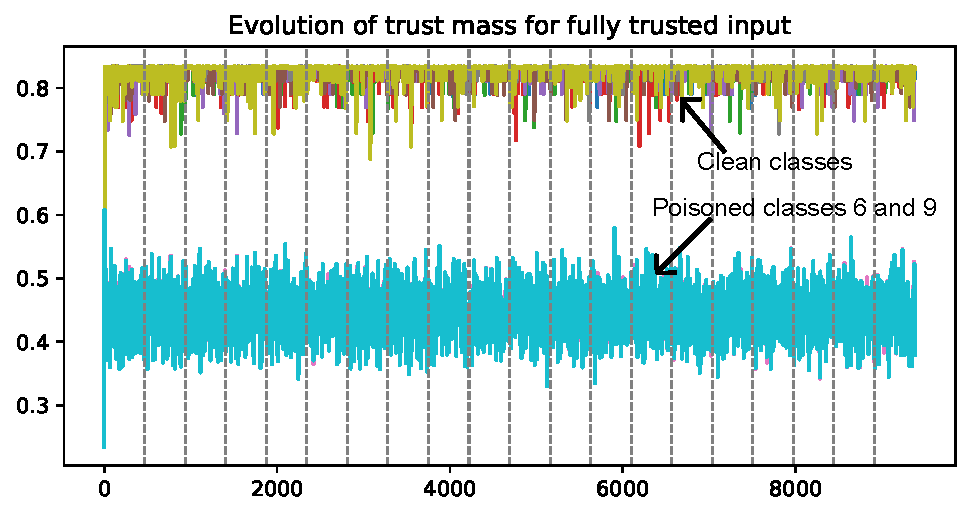
\includegraphics[width=\linewidth]{img/patas/plot_ptas-128-t-t-ps4.pdf}
    \caption{Evolution of trust masses across training rounds (one round corresponds to a feedforward and backpropagation pass).}
    \end{subfigure}
    \begin{subfigure}{0.45\linewidth}
        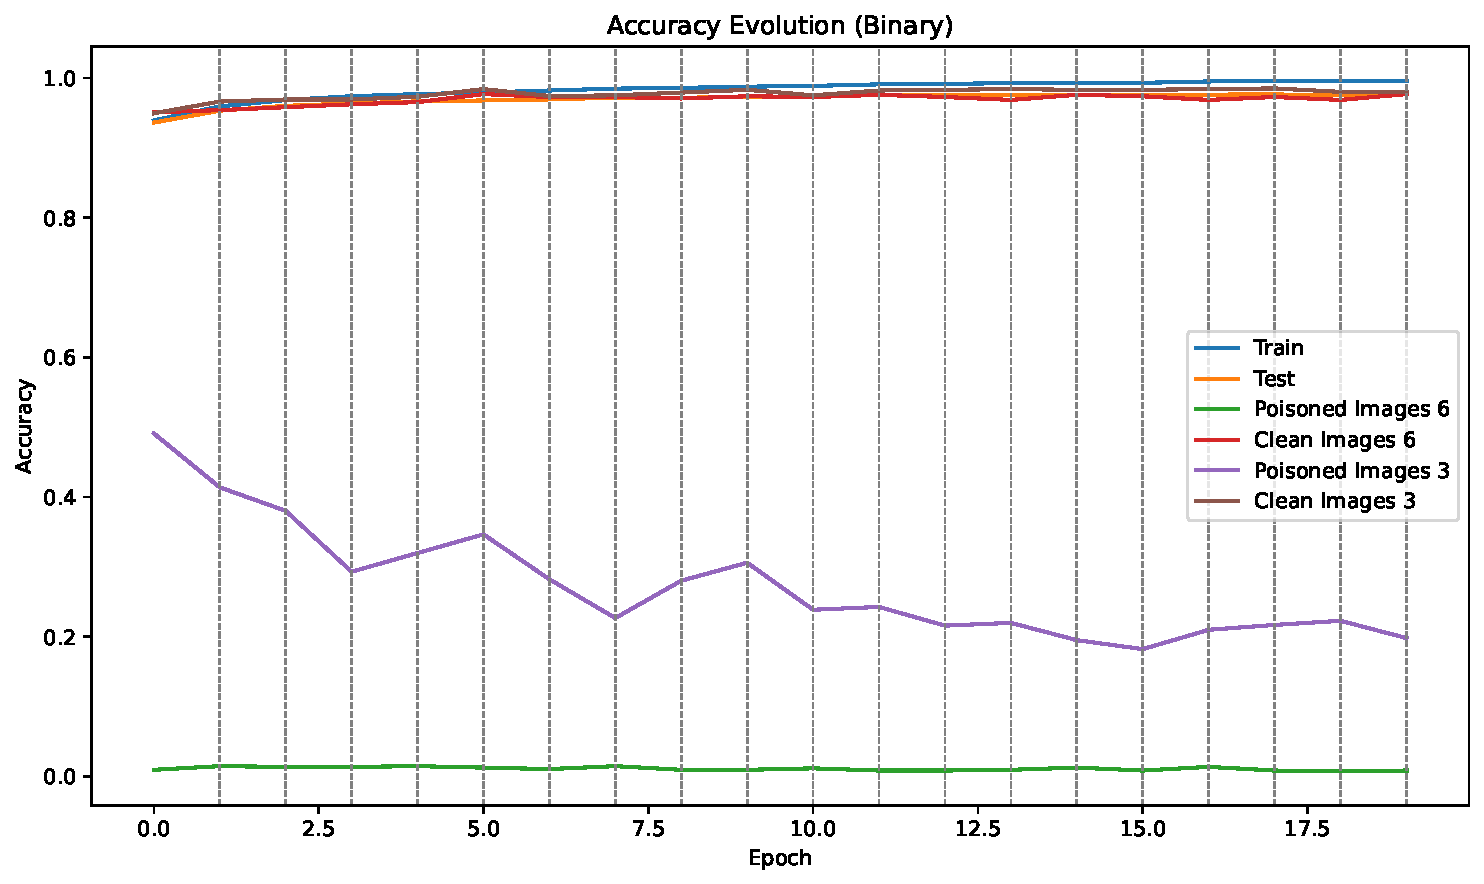
\includegraphics[width=\linewidth]{latex/NN_Train_mnist_128_trust_trust_PathSize_4__accuracy_evolution.pdf}
    \caption{Accuracy}
    \end{subfigure}
    \caption{Evolution of trust mass for fully trusted input in the MNIST poisoned Experiment with patch size \(4\times 4\) pixels}
    \label{fig:4x4}
\end{figure}
The evaluation of the Parallel Trust Assessment System (PaTAS) is conducted during the training phase of the \ac{NN}. After each iteration of training (i.e., a complete feedforward and backpropagation cycle), we assume that an inference is performed, and we assess the trustworthiness of the corresponding output. This assessment is carried out under three input trust profiles:
\begin{itemize}
\item \emph{Fully Trusted Input}: input is considered fully trusted.
\item \emph{Fully Uncertain Input}: input is considered fully uncertain.
\item \emph{Fully Distrusted Input}: input is fully unreliable.
\end{itemize}
We focus on these three profiles because they represent the extreme and most informative boundary cases of input trust. 

For each of these three input types, we track and plot the evolution of three key metrics over the course of training:
\begin{itemize}
\item \emph{Trust Mass}: the level of confidence in the output.
\item \emph{Uncertainty Mass}: the uncertainty of the assessment.
\item \emph{Distrust Mass}: the level of disbelief in the output.
\end{itemize}

As a result, for each evaluation, 9 distinct plots are generated, corresponding to the 3 input types (fully trusted, fully uncertain, and fully distrusted) and each of the three key metrics (trust, uncertainty, and distrust)\footnote{The base rate is set to 0.5 and remains constant across all experiments.}.

All the results are depicted in Figures in the \appp and summarized in \cref{tab:cancer_results,tab:mnist,tab:mnistpois,fig:mnistpoisipta}. They confirm several theoretical properties of \ac{PaTAS-TP} proven in \cref{sec:ptastheory}:



\begin{itemize}
\item \emph{Convergence of Trust Assessment}: when accuracy converges, trust assessment converges as expected.
\item \emph{Inference on fully uncertain input yields fully uncertain output}: a fully uncertain input always produces a fully uncertain output.
\item \emph{Symmetric Inference}: when input trust assessments are symmetric, the inference results remain symmetric.
\end{itemize}

For detailed results, we primarily focus on the three plots for each experiment) corresponding to feedforward of fully trusted input. Processing uncertain inputs naturally yields uncertain outputs, while symmetry implies that trusted and distrusted cases mirror each other. We also confirm that when processing fully trusted inputs, the distrust mass remains close to zero. Since trust, uncertainty, and distrust sum to 1, analyzing only the trust mass is sufficient in such cases. Therefore we keep only the trust mass after the training in \cref{tab:cancer_results,tab:mnist,tab:mnistpois,tab:epsilon_gap}. 

\subsubsection*{Experiment 1 -- Breast Cancer Classification}
\begin{table}[ht]
\resizebox{\textwidth}{!}{%
\begin{tabular}{llcccccc}
\hline
X Trust & Y Trust & $\epsilon=1$ & $\epsilon=0.1$ & $\epsilon=0.01$ & $\epsilon=0.001$ & Train (\%) & Test (\%) \\
\hline
trust & trust & 0.8787 & 0.8787 & 0.6658 & 0.1681 & 98.68 & 96.49 \\
trust & vacuous & 0.3242 & 0.2927 & 0.1290 & 0.0773 & 65.71 & 74.56 \\
trust & distrust & 0.00 & 0.00 & 0.00 & 0.00 & 99.12 & 2.63 \\
vacuous & trust & 0.3392 & 0.3392 & 0.2682 & 0.0931 & 96.70 & 95.61 \\
vacuous & vacuous & 0.3051 & 0.2971 & 0.1820 & 0.1034 & 68.79 & 88.60 \\
vacuous & distrust & 0.00 & 0.00 & 0.00 & 0.00 & 96.92 & 4.39 \\
distrust & trust & 0.00 & 0.00 & 0.00 & 0.00 & 64.62 & 43.86 \\
distrust & vacuous & 0.00 & 0.00 & 0.00 & 0.00 & 56.92 & 33.33 \\
distrust & distrust & 0.00 & 0.00 & 0.00 & 0.00 & 65.49 & 40.35 \\
\hline
\multicolumn{8}{c}{\textit{Extra scenarios}} \\
\hline
(0.25, 0.25, 0.5) & (0.25, 0.25, 0.5) & 0.1172 & 0.1140 & 0.0633 & 0.0272 & 68.79 & 88.60 \\
(0.25, 0.0, 0.75) & (0.25, 0.0, 0.75) & 0.3810 & 0.3809 & 0.2211 & 0.0871 & 80.22 & 95.61 \\
\hline
\end{tabular}%
}
\caption{Summary of final trust mass across four values of $\epsilon$ and corresponding train/test accuracies for the Breast Cancer Classification Experiment.}
\label{tab:cancer_results}
\end{table}

The results for this experiment are summarized in \cref{tab:cancer_results}. When both features and labels are clean, the model steadily improves and achieves high accuracy (98.68\% training, 97.69\% test), and \ac{PaTAS-TP} produces the highest trust mass across all conditions (0.88 for $\epsilon=0.1$). Clean features with corrupted labels cause test accuracy to collapse to 2.63\%, even while training accuracy remains artificially high at 99.12\%; the model learns the wrong mapping but does so confidently. Correspondingly, trust mass falls to zero regardless of $\epsilon$, correctly signaling the unreliability of the learned parameters. With vacuous labels, performance degrades moderately (65.71\% train, 74.56\% test) and trust mass remains low (0.29). Corrupted features eliminate the ability to learn in any combination: trust mass is zero in all distrust-$X$ rows and test accuracy never exceeds 43.86\%. 

The mild-degradation scenario $(0.25, 0, 0.75)$ for features and labels is the only intermediate case and behaves as expected: with only 15\% of features perturbed and no distrust component, trust mass reaches 0.38 for $\epsilon=0.1$, outperforming every row that uses a fully vacuous opinion for either features or labels. This suggests that an analyst who can bound the degradation and express it as a partial-trust opinion, rather than defaulting to full uncertainty, obtains a more optimistic trust assessment.

We evaluated the system for four values of $\epsilon$ ($0.001, 0.01, 0.1, 1$). We recall that $\epsilon$ is the threshold used by the \textsc{NodeTrust} function in \cref{alg:trustupdate}.
\begin{itemize}
\item For $\epsilon = 0.01$: the system is more sensitive to gradient magnitude. Fully trusted $X$ with trusted $Y$ yields a trust mass of 0.67, while uncertain $Y$ reduces it to 0.13. When $X$ is vacuous, trust stabilizes around 0.27 for trusted $Y$ and 0.18 for uncertain $Y$.
\item For $\epsilon = 0.1$: the larger threshold makes the system less reactive to small gradients. Fully trusted $X$ with trusted $Y$ reaches 0.88; with uncertain $Y$, trust falls to 0.29. Vacuous $X$ with trusted $Y$ yields 0.34, and with uncertain $Y$ yields 0.30. In all cases, distrust in either $X$ or $Y$ drives trust mass to zero.
\end{itemize}

The two additional values clarify the boundary behavior of $\epsilon$. At $\epsilon = 0.001$, the threshold falls well below the typical gradient magnitude during training, causing \textsc{NodeTrust} to classify nearly all gradients as large and therefore as negative evidence; trust mass collapses across all non-distrust configurations, losing the ability to differentiate between trust profiles. At $\epsilon = 1$, the threshold is so permissive that almost all gradients are treated as small, producing results nearly identical to $\epsilon = 0.1$ and offering no additional discriminative power. Among the four values evaluated, $\epsilon = 0.1$ emerges as the most balanced choice, maintaining sensitivity to meaningful gradient activity without collapsing trust mass or losing discriminative power. How $\epsilon$ should be set in practice is discussed in \cref{sec:patas-discussion}.

A notable observation is that the \textit{trust/vacuous} configuration yields a lower trust mass than \textit{vacuous/vacuous} across all values of $\epsilon$ except $\epsilon = 1$. This ordering is consistent with the test accuracies reported in \cref{tab:cancer_results}, where \textit{trust/vacuous} (74.56\%) underperforms \textit{vacuous/vacuous} (88.60\%). The underlying mechanism is that trusted features produce strong, informative gradients that frequently exceed $\epsilon$, generating negative evidence in \textsc{NodeTrust} when labels are unreliable: the model confidently learns from clean features under vacuous supervision, effectively fitting an unreliable mapping. Noisy features, by contrast, produce diffuse gradients that remain below $\epsilon$ more often, partially canceling the effect of uncertain labels and yielding comparatively higher trust mass. This shows that smaller values of $\epsilon$ correctly capture this ordering, while $\epsilon = 1$ is too permissive to discriminate between these regimes and the effect vanishes.

Overall, there is a strong positive correlation between trust mass and test accuracy. Moreover, a smaller $\epsilon$ makes label trust more influential: the relative gap between trusted-$Y$ and uncertain-$Y$ rows, defined as $(T_{\text{trusted}} - T_{\text{uncertain}}) / T_{\text{trusted}}$,
increases as $\epsilon$ decreases, as shown in \cref{tab:epsilon_gap}.
\begin{table}[h]
\centering
\caption{Relative influence of label trust as a function of $\epsilon$,
for trusted and vacuous feature inputs.}
\label{tab:epsilon_gap}

\begin{tabular}{lcccc}
\hline
 & \multicolumn{2}{c}{$\epsilon = 0.1$} & \multicolumn{2}{c}{$\epsilon = 0.01$} \\
\cmidrule(lr){2-3}\cmidrule(lr){4-5}
$X$ trust & $T_{Y=\text{trust}}$ & $T_{Y=\text{vac}}$ & $T_{Y=\text{trust}}$ & $T_{Y=\text{vac}}$ \\
\hline
trusted  & 0.88 & 0.29 & 0.67 & 0.13 \\
vacuous  & 0.34 & 0.30 & 0.27 & 0.18 \\
\hline
\multicolumn{5}{l}{\small Relative gap (trusted): $(0.88-0.29)/0.88 = 67\%$ vs $(0.67-0.13)/0.67 = 81\%$} \\
\multicolumn{5}{l}{\small Relative gap (vacuous): $(0.34-0.30)/0.34 = 12\%$ vs $(0.27-0.18)/0.27 = 33\%$} \\
\hline
\end{tabular}
\end{table}


\begin{tcolorbox}[title=Key findings -- Experiment 1, colback=gray!5, colframe=gray!40, fonttitle=\bfseries, left=4pt, right=4pt, top=4pt, bottom=4pt]
\textbf{F1.1 Label trust matters more than feature trust.} Setting $X$ as vacuous
while keeping $Y$ trusted yields a higher trust mass (0.34) than the reverse
(0.29 for trusted $X$, uncertain $Y$).

\medskip
\textbf{F1.2 Distrust is more damaging than uncertainty.} Replacing a fully
uncertain opinion $(0,0,1)$ for both $X$ and $Y$ with a mixed assessment
$(0.25, 0.25, 0.5)$ reduces trust mass from 0.30 to 0.11, while accuracy
remains unchanged (88.60\%), confirming the drop is driven by the distrust
component alone.

\medskip
\textbf{F1.3 Finer $\epsilon$ amplifies label-trust sensitivity.} As shown in
\cref{tab:epsilon_gap}, the relative gap between trusted-$Y$ and uncertain-$Y$
is larger for $\epsilon=0.01$ than for $\epsilon=0.1$, in both the trusted and
vacuous feature settings.
\end{tcolorbox}














\subsubsection*{Experiment 2 -- MNIST Dataset}
\begin{table}
\centering
\begin{tabular}{cccccc}
\hline
Architecture & X Trust & Y Trust & Trust Mass & Train Acc (\%) & Test Acc (\%) \\
\hline
16 & vacuous & vacuous & 0.3087 & 65.19 & 73.96 \\
32 & vacuous & vacuous & 0.3224 & 66.20 & 79.03 \\
64 & vacuous & vacuous & 0.3306 & 67.22 & 89.98 \\
128 & vacuous & vacuous & 0.3359 & 67.78 & 92.05 \\
16-16 & vacuous & vacuous & 0.1628 & 65.68 & 69.39 \\
16 & trust & trust & 0.8620 & 96.37 & 95.13 \\
16-16 & trust & trust & 0.7077 & 96.83 & 95.84 \\
\hline
\end{tabular}
\caption{Summary of final trust mass for the MNIST Classification Experiment.}
\label{tab:mnist}
\end{table}
In this experiment, \ac{PaTAS-TP} produces ten output trust opinions, one for each class. However, they are almost identical across classes, so we record only the aggregated trust mass in \cref{tab:mnist}.

When features and labels are vacuous, accuracy improves as model size increases, from 73.96\% (architecture 16) to 92.05\% (architecture 128). Test accuracy consistently exceeds training accuracy across all architectures, suggesting that training under vacuous trust makes the model underestimate its own learning progress. Trust mass follows the same upward trend with model size (0.3087, 0.3224, 0.3306, 0.3359), though the gains become progressively smaller, indicating diminishing returns from added capacity under uncertain data.

The two-layer architecture (16-16) is a notable exception. Despite having more parameter count than the single-layer 16-hidden neurons network, it yields a trust mass of only 0.1628 under vacuous inputs and 0.7077 under trusted inputs, both consistently lower than the single-layer 16-neuron counterpart (0.3087 and 0.8620 respectively). This is not an artifact but a meaningful property of the framework: each additional layer introduces an extra round of trust discounting, which attenuates the trust signal propagating through the network. A deeper architecture therefore inherits less trust from its inputs, even when those inputs are reliable. This behavior is consistent with \ac{PaTAS-TP} design, since a deeper inference path involves more parameters, each contributing uncertainty, and the framework correctly reflects that the output trust depends on the full chain of parameter reliability. A secondary factor is convergence speed: deeper networks require more epochs to stabilize their gradients, so the parameter trust opinions accumulate evidence more slowly and remain closer to their vacuous initialization at the end of training.

The trusted evaluation provides the clearest contrast. Architecture 16 with trusted features and labels reaches a trust mass of 0.8620, far exceeding any vacuous-data configuration regardless of architecture size. Even the deeper 16-16 architecture achieves 0.7077 under trusted inputs, outperforming the largest single-layer architecture (128, trust mass 0.3359) trained under vacuous data by a wide margin. This confirms that data quality has a far greater impact on the resulting trust assessment than model capacity.

\begin{tcolorbox}[title=Key findings -- Experiment 2, colback=gray!5,
colframe=gray!40, fonttitle=\bfseries, left=4pt, right=4pt,
top=4pt, bottom=4pt]

\textbf{F2.1 Trust increases with model width, with diminishing returns.} Under vacuous data, trust mass grows from 0.3087 (16 neurons) to 0.3359 (128 neurons), but the incremental gain shrinks at each step, suggesting that additional capacity provides less benefit once the dominant bottleneck is data quality rather than model expressiveness.

\medskip
\textbf{F2.2 Depth penalises trust due to discounting accumulation.} The 16-16 architecture consistently yields lower trust than the single-layer 16-neuron network under both vacuous (0.1628 vs.\ 0.3087) and trusted (0.7077 vs.\ 0.8620) inputs. Each additional layer introduces an extra discounting step, so deeper networks attenuate the trust signal regardless of their predictive accuracy.

\medskip
\textbf{F2.3 Data quality dominates model capacity for trust.} Training the smallest architecture on trusted data (trust mass 0.8620) far exceeds training the largest architecture on vacuous data (trust mass 0.3359). Investing in data quality is therefore more beneficial for trust than scaling the model.
\end{tcolorbox}


\subsubsection*{Experiment 3 -- Poisoned MNIST Dataset}
\begin{table}[ht]
\centering
\resizebox{\textwidth}{!}{
\begin{tabular}{ccccccccc}
\hline
Patch size & Trust for 3 & Trust for 6 & Train (\%) & Test (\%) & Clean 3 (\%) & Clean 6 (\%) & 3 with patch (\%) & 6 with patch (\%) \\
\hline
$(1 \times 1)$   & 0.836 & 0.440 & 99.62 & 97.66 & 97.72 & 97.49 & 83.76 & 0.63 \\
$(4 \times 4)$   & 0.833 & 0.439 & 99.62 & 97.66 & 98.02 & 97.70 & 19.80 & 0.84 \\
$(10 \times 10)$ & 0.815 & 0.433 & 99.60 & 97.61 & 97.62 & 97.49 & 16.44 & 0.63 \\
$(27 \times 27)$ & 0.651 & 0.386 & 96.35 & 97.73 & 98.02 & 97.81 &  0.00 & 0.00 \\
\hline
\end{tabular}
}
\caption{Summary of results for the Poisoned MNIST Classification Experiment.}
\label{tab:mnistpois}
\end{table}


\begin{figure}
    \centering
    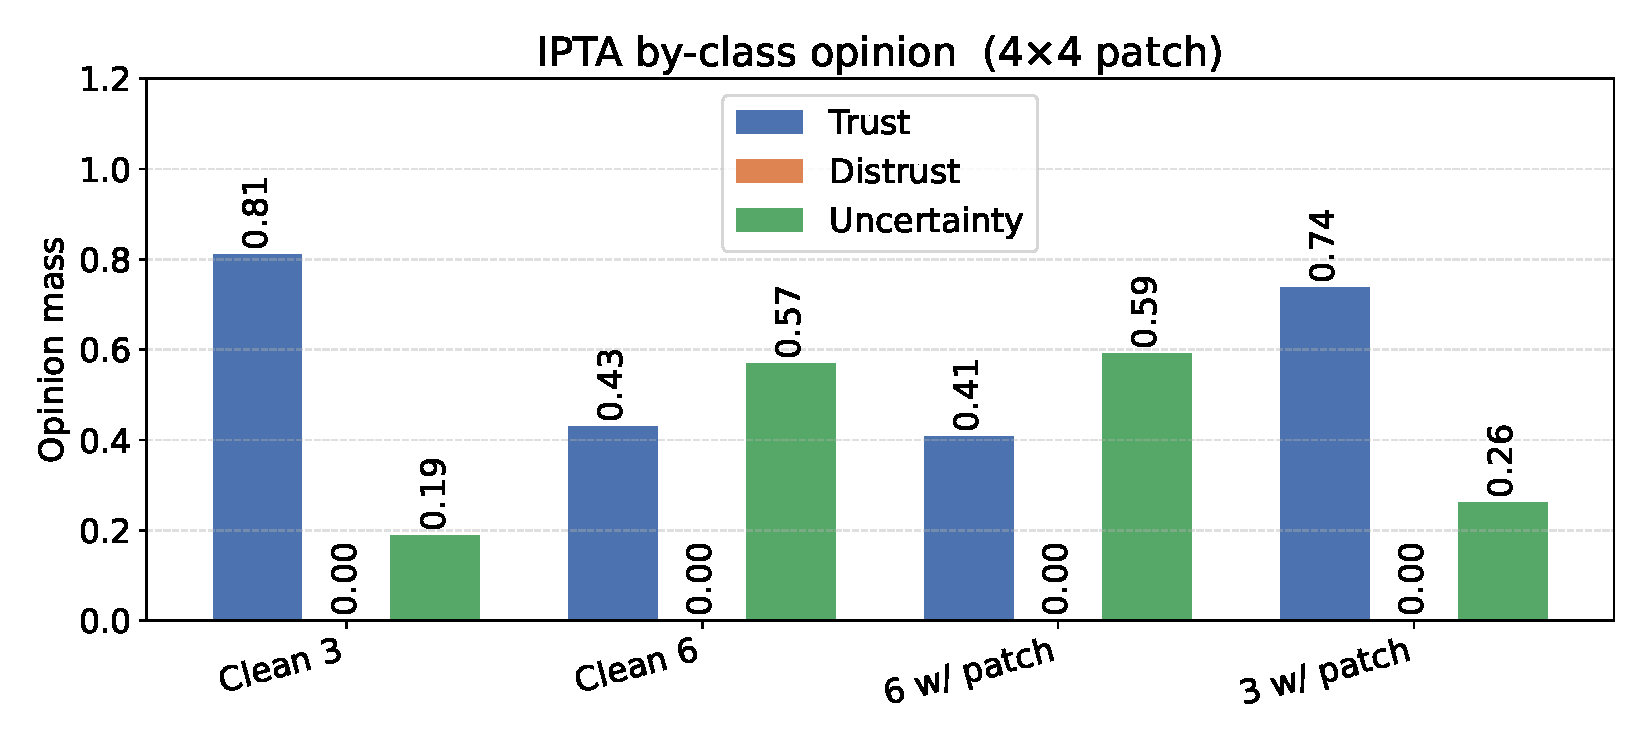
\includegraphics[width=0.8\linewidth]{latex/NN_Train_mnist_128_trust_trust_PathSize_4__ipta_table2a.pdf}
    \caption{\ac{IPTA} results for \ac{NN} trained on poisoned datasets with patch size $4 \times 4$. Results are obtained by feedforwarding a fully trusted opinion, except the patch-distrusted, where patch pixels are explicitly assigned distrust.}
    \label{fig:mnistpoisipta}
\end{figure}

\begin{table}[h]
\centering
\caption{Relative trust gap between clean label 3 and poisoned label 6
as a function of patch size.}
\label{tab:reldrop}
\begin{tabular}{lccc}
\hline
Patch size & $T_3$ & $T_6$ & $(T_3 - T_6)/T_3$ (\%) \\
\hline
$1\times1$   & 0.836 & 0.440 & 47.4 \\
$4\times4$   & 0.833 & 0.439 & 47.3 \\
$10\times10$ & 0.815 & 0.433 & 46.9 \\
$27\times27$ & 0.651 & 0.386 & 40.7 \\
\hline
\end{tabular}
\end{table}

As in the previous experiment, \ac{PaTAS-TP} produces ten output trust opinions. In \cref{tab:mnistpois} we report the trust mass for label 3 (a clean class) and label 6 (a poisoned class), alongside overall train/test accuracy and per-class accuracy on both clean and patched test samples.

Across all patch sizes, the trust mass for label 3 consistently exceeds that for label 6 (e.g.\ 0.836 vs.\ 0.440 for the $1\times1$ patch), confirming that \ac{PaTAS-TP} reliably distinguishes clean from poisoned labels even when overall accuracy remains high (97.66\%). As the patch grows, both trust values decrease, but not symmetrically: as shown in \cref{tab:reldrop}, the relative gap $(T_3 - T_6)/T_3$ decreases with patch size, from 47.4\% at $1\times1$ down to 40.7\% at $27\times27$, indicating that larger patches erode the trust advantage of the clean class more than they further penalize the already-distrusted poisoned class. As a result, the gap between the two patches decreases with patch size. This asymmetry is interpretable: as the patch occupies a larger fraction of the image, the underlying model increasingly associates the patch pattern directly with the target poisoned class, bypassing the remaining image features. The parameters involved in clean-class prediction are therefore affected more by the growing patch than those already conditioned on the poisoned signal, which partially absorbs the patch regardless of its size. The clear separation between the two classes is nonetheless maintained across all patch sizes.

Regarding classification accuracy, patched digit 6 samples are almost entirely misclassified regardless of patch size ( $\leq$ 0.84\%), confirming the backdoor
attack is effective. Patched digit 3 accuracy degrades more gradually, dropping
sharply from 83.76\% at $1\times1$ to roughly 16 to 20\% for larger patches,
reflecting the spatial overlap between the patch and discriminative features for
digit 3. The $27\times27$ case is an edge case rather than a realistic poisoning
scenario: a patch of this size dominates the entire image at inference time, so
the model associates the input almost entirely with the poisoned trigger rather
than the digit. One of the poisoned classes therefore reaches near-100\% accuracy
while the other collapses to 0\%, producing the 0\% accuracy observed for both
patched digits 3 and 6. This extreme case is included only to illustrate the
boundary behavior of the framework.

To evaluate the \ac{IPTA}, \cref{fig:mnistpoisipta} reports accuracy and the full trust opinion $(t, d, u)$ for clean and patched samples, obtained by feedforwarding a fully trusted opinion through the \ac{IPTA} instantiated from the respective inference path in the $4\times 4$ patch model. As established in \cref{thm:infvac} (Remark~7.1), feedforwarding a fully trusted input $(1, 0, 0)$ through any \ac{PaTAS-TP} configuration yields an output with zero distrust mass, since the discounting operator maps a fully trusted input to an opinion with $d=0$, and fusion preserves this zero mass. This is confirmed across all rows using a trusted $T_x$: distrust remains exactly 0 in every case.

Clean digit 3 achieves the strongest trust profile (0.811 trust, 0.189 uncertainty), consistent with high accuracy (98.02\%). Clean digit 6 already exhibits markedly higher uncertainty (0.570) despite comparable accuracy (97.70\%), reflecting that the parameters on the digit-6 inference path were exposed to poisoned training samples and are therefore less trusted.

For patched samples, the degradation is clear. Patched digit 6 accuracy collapses to 0.84\% and trust drops to 0.408, with uncertainty dominating at 0.592, providing a warning signal unavailable from accuracy alone. For patched digit 3, accuracy falls to 19.80\% yet trust remains relatively higher at 0.738, reflecting that the digit-3 inference path passes through less poisoned parameters. \DIFaddbegin \DIFadd{A ten-training replication of this setup under the released implementation, with only the evaluation seed varied, confirms the gap is robust: mean }\ac{IPTA} \DIFadd{trust $0.884 \pm 0.001$ for the clean class against $0.503 \pm 0.035$ for the poisoned class. Two assumptions of this experiment, the oracle knowledge of the patch location in the trust assignment and the joint application of patch and label flip, are removed in Experiment~4, which detects the same poisoning with estimated input opinions and separates the two corruption channels. 
}\DIFaddend 

\begin{tcolorbox}[title=Key findings -- Experiment 3, colback=gray!5,
colframe=gray!40, fonttitle=\bfseries, left=4pt, right=4pt,
top=4pt, bottom=4pt]

\textbf{F3.1 Trust separates clean from poisoned inference paths.} Across all patch sizes, the trust mass for label 3 (clean) consistently exceeds that for label 6 (poisoned), even when overall test accuracy remains above 97\%. \ac{PaTAS-TP} therefore reveals reliability differences that accuracy alone cannot expose.

\medskip
\textbf{F3.2 Larger patches narrow the trust gap by affecting clean paths
more than poisoned ones.} As patch size grows, the trust mass for the clean label decreases more steeply than for the poisoned label. The model increasingly relies on the patch pattern rather than image features, which degrades the parameters along clean-class inference paths more than those already conditioned on
the poisoned signal.

\medskip
\textbf{F3.3 Zero distrust under trusted input is theoretically guaranteed.} When the input trust is fully trusted $(1,0,0)$, distrust in the output is exactly zero, as established in \cref{thm:infvac}. This is confirmed empirically across all IPTA rows using trusted $T_x$.
\end{tcolorbox}

These results demonstrate that \ac{PaTAS-TP} not only correlates with accuracy but provides complementary information: it identifies which inference paths are structurally less reliable, responds to the size of adversarial corruption, and distinguishes clean from poisoned classes even when overall accuracy remains high.

\DIFaddbegin \subsubsection*{\DIFadd{Experiment 4 -- Comparative Trust Evaluation}}

\paragraph*{\DIFadd{In-distribution behavior.}}
\DIFadd{On clean test data the composed score matches the maximum-softmax filter on correct-versus-incorrect discrimination (AUROC $0.979 \pm 0.003$ for both on MNIST), with equal calibration error after identical post-hoc calibration: when nothing violates the training distribution, trust-weighting costs nothing. Under corruption the two signals separate }\emph{\DIFadd{by design}}\DIFadd{: accuracy barely drops on the robust MLP, so the softmax retains a higher correct-versus-incorrect AUROC on the mixed batch ($0.974$ vs.\ $0.895$) precisely because it ignores the distribution violation that the trust factor flags. Confidence ranks correctness within the training distribution; trust exposes inputs that leave it. The detection tasks below measure the latter.
}

\begin{table}[ht]
\centering
\resizebox{\textwidth}{!}{%
\begin{tabular}{lcccccc}
\hline
 & OOD M$\to$F & Det.\ MNIST & Det.\ F-MNIST & OOD F$\to$M & Shift & Blend \\
Method & AUROC & AUROC & AUROC & AUROC & AUROC & AUROC \\
\hline
PaTAS (composed) & 0.975 & 0.972 & 0.835 & 0.781 & \textbf{0.781} & 0.564 \\
Conformity alone & \textbf{1.000} & \textbf{1.000} & \textbf{0.994} & 0.481 & 0.678 & 0.500 \\
Mahalanobis (pixel) & 0.997 & 0.997 & 0.944 & 0.942 & 0.716 & 0.482 \\
kNN (pixel) & 0.965 & 0.603 & 0.707 & 0.967 & 0.749 & 0.500 \\
Mahalanobis (feature) & 0.978 & 0.743 & 0.785 & \textbf{0.988} & 0.783 & 0.474 \\
kNN (feature) & 0.994 & 0.588 & 0.625 & 0.973 & \textbf{0.801} & 0.508 \\
Energy score & 0.850 & 0.636 & 0.603 & 0.873 & 0.707 & 0.541 \\
Max softmax & 0.883 & 0.631 & 0.558 & 0.805 & 0.740 & 0.566 \\
MC Dropout & 0.936 & 0.621 & 0.545 & 0.834 & 0.747 & 0.574 \\
\ac{EDL} & 0.883 & 0.547 & 0.510 & 0.767 & 0.736 & 0.561 \\
\hline
\end{tabular}%
}
\caption{\DIFaddFL{Detection of distribution violations (mean over three evaluation seeds, dispersion at most $\pm 0.005$): }\ac{OOD} \DIFaddFL{detection in both directions between MNIST and Fashion-MNIST, clean-versus-corrupted separation on the mixed batches (uniform feature noise), and the two hard MNIST corruptions (marginal-preserving translation; low-amplitude blended center trigger). The blended trigger defeats every method (best entry $0.574$), an honest limit of all ten scores against an adversary that stays inside the per-feature range.}}
\label{tab:diss-detection}
\end{table}

\paragraph*{\DIFadd{Detection and attribution.}}
\Cref{tab:diss-detection} \DIFadd{reports the violation-detection tasks. Three mechanisms are cleanly separable. First, }\emph{\DIFadd{violation detection is carried by input-space signals}}\DIFadd{: the conformity opinions are perfect or near-perfect where inputs violate the training marginals (}\ac{OOD} \DIFadd{M$\to$F $1.000$, corruption detection $1.000$ and $0.994$), the raw-pixel Mahalanobis baseline is close behind, and an ablation replacing the conformity opinions with the constant fully trusted opinion collapses the composed score to the output-only level ($0.896$ and $0.639$ on the forward tasks, single-seed). Trust propagation is not the detector; it is the carrier that turns the detection signal into an opinion composable with model trust. Second, }\emph{\DIFadd{propagation contributes exactly where the input marginals are silent}}\DIFadd{: under the marginal-preserving translation the conformity score drops to $0.678$ as predicted by its construction, while the composed score reaches $0.781$, above its own input factor, because translated inputs traverse atypical activation paths that the }\ac{IPTA} \DIFadd{reads as less trusted. Third, }\emph{\DIFadd{the directions of failure are principled}}\DIFadd{: in the subset direction (Fashion-MNIST model, MNIST digits as }\ac{OOD}\DIFadd{), digits occupy a quiet subset of the clothing marginals rather than violating them, the conformity score collapses below chance ($0.481$), and the neighborhood- and covariance-based detectors own the task ($0.988$ feature Mahalanobis, $0.942$ pixel Mahalanobis). The composition fails safely there: the confidence factor keeps the composed score at the output-baseline level ($0.781$ vs.\ $0.805$ softmax) instead of inheriting the collapse. Since the subset-direction signal demonstrably exists in input space, mapping such a detector through the same quantification into an additional input opinion is a natural }\ac{SL} \DIFadd{extension, left as future work.
}

\DIFadd{On the applicability-boundary case, GTSRB, the marginal conformity model detects corruption only weakly ($0.645$; composed $0.545$), exactly as the diagnostics of }\cref{sec:conformity} \DIFadd{predict (}\cref{tab:diss-diagnostics}\DIFadd{: no witness features with $w_j \geq 4$). The pixel-space Mahalanobis baseline still reaches $0.997$ on the same task: the boundary belongs to the per-feature marginal model, not to input-space assessment as such, which sharpens the diagnostics into an actionable gate: when they flag a domain, a covariance-aware input model is required.
}

\begin{table}[ht]
\centering
\begin{tabular}{lccccc}
\hline
\DIFaddFL{Dataset }& \DIFaddFL{Med.\ $\sigma_{\mathrm{eff}}$ }& \DIFaddFL{$w_{\max}$ }& \DIFaddFL{Top-10\% }& \DIFaddFL{$w{\geq}4$ }& \DIFaddFL{Det. }\\
\hline
\DIFaddFL{MNIST }& \DIFaddFL{0.47 }& \DIFaddFL{52.3 }& \DIFaddFL{0.32 }& \DIFaddFL{0.40 }& \DIFaddFL{0.972 }\\
\DIFaddFL{Fashion-MNIST }& \DIFaddFL{0.90 }& \DIFaddFL{64.0 }& \DIFaddFL{0.76 }& \DIFaddFL{0.18 }& \DIFaddFL{0.835 }\\
\DIFaddFL{GTSRB }& \DIFaddFL{0.98 }& \DIFaddFL{1.8 }& \DIFaddFL{0.14 }& \DIFaddFL{0.00 }& \DIFaddFL{0.545 }\\
\DIFaddFL{CIFAR-10 (gray) }& \DIFaddFL{0.23 }& \DIFaddFL{1.1 }& \DIFaddFL{0.11 }& \DIFaddFL{0.00 }& \DIFaddFL{-- }\\
\hline
\end{tabular}
\caption{\DIFaddFL{A-priori applicability diagnostics of the conformity model, computed on clean training features before any model is trained (median effective deviation, maximum reliability weight, weight share of the top decile, fraction of features with $w_j \geq 4$), against the composed score's corruption detection later observed. Registered domains concentrate evidence in reliable witnesses; unregistered imagery has none, and the input-side signal is predicted, and confirmed, to be uninformative there.}}
\label{tab:diss-diagnostics}
\end{table}

\paragraph*{\DIFadd{Poisoning without an oracle.}}
\DIFadd{The conformity opinions remove the oracle assumption of Experiment~3. Fed unchanged into the poisoned model's }\ac{IPTA}\DIFadd{, they flag patched inputs with no knowledge of the trigger: the input trust alone separates clean from patched inputs at AUROC $1.000$ for both classes, because the patch violates the near-constant border features the conformity model weights most, and the parameter-side gap between the clean and poisoned class persists under these estimated opinions (trust $0.780$ vs.\ $0.499$; oracle assignment $0.871$ vs.\ $0.559$). The remaining assumption, a clean feature source for the conformity fit, degrades gracefully: fitting on the poisoned training set itself still detects the trigger at $0.73$ and $0.67$ per class, while a naive robust fit (median and MAD) does not recover ($0.65$), since MNIST pixel marginals are zero-inflated; contamination-aware conformity fits are explicit future work.
}

\paragraph*{\DIFadd{Separating the corruption channels.}}
\DIFadd{Experiment~3 applies patch and label flip jointly. Single-channel controls retrained at the paper's patch size separate their effects on the per-class output trust (}\cref{tab:diss-classtrust}\DIFadd{): under the full backdoor both flipped classes carry an identical trust deficit ($0.756$ for digits 6 and 9 alike, $0.19$ below the minimum of the eight clean classes, whose spread is below $0.001$); the label-flip-only control reproduces nearly the full drop ($0.748$), the patch-only control still produces a clearly detectable deficit ($0.788$), and the unpoisoned model shows no false alarm (both classes at the clean level $0.994$). The trust deficit is therefore pair-specific, symmetric across the flipped pair, driven primarily by the label channel, and present for a purely spurious trigger even when every label is correct.
}

\begin{table}[ht]
\centering
\begin{tabular}{lcccc}
\hline
\DIFaddFL{Training condition }& \DIFaddFL{Clean-class mean }& \DIFaddFL{Clean-class min }& \DIFaddFL{Trust$_6$ }& \DIFaddFL{Trust$_9$ }\\
\hline
\DIFaddFL{Unpoisoned }& \DIFaddFL{0.994 }& \DIFaddFL{0.994 }& \DIFaddFL{0.994 }& \DIFaddFL{0.994 }\\
\DIFaddFL{Full backdoor (patch + flip) }& \DIFaddFL{0.947 }& \DIFaddFL{0.946 }& \DIFaddFL{0.756 }& \DIFaddFL{0.756 }\\
\DIFaddFL{Label flip only }& \DIFaddFL{0.947 }& \DIFaddFL{0.947 }& \DIFaddFL{0.748 }& \DIFaddFL{0.747 }\\
\DIFaddFL{Trigger patch only }& \DIFaddFL{0.948 }& \DIFaddFL{0.948 }& \DIFaddFL{0.788 }& \DIFaddFL{0.788 }\\
\hline
\end{tabular}
\caption{\DIFaddFL{Per-class output trust (projected probability under a fully trusted input) for the $4\times4$ poisoned MNIST setup and its single-channel controls (784-128-10). Both flipped classes drop identically and far outside the clean-class band; the label channel carries most of the deficit, and the spurious patch alone remains detectable.}}
\label{tab:diss-classtrust}
\end{table}

\paragraph*{\DIFadd{Training-quality audit.}}
\DIFadd{The model-side trust provides a training-quality audit that requires no test data at all (}\cref{tab:diss-audit}\DIFadd{). Under increasing train-time label-flip rates $p$, the feedforward trust under a fully trusted input drops by $31.7\%$ relative to the clean-trained model at }\emph{\DIFadd{any}} \DIFadd{non-zero rate, including $p = 0.1$ where test accuracy moves by only three points: a corruption tripwire read from the trained trust state alone. The flat level is designed saturation, not an artifact: at $p = 0.1$ essentially every training batch already contains corrupted labels, so every batch delivers the large-gradient corrections that }\textsc{\DIFadd{NodeTrust}} \DIFadd{counts as negative evidence, and the converged trust registers }\emph{\DIFadd{that}} \DIFadd{corruption is present rather than how much. When the algorithm instead consumes rate-informed label opinions $T_y = (1{-}p, 0, p)$, the same machinery grades monotonically ($0.951 \to 0.805$): tripwire versus graded meter is a property of the label opinion's informativeness, not of the calculus. The scale-tied threshold of }\cref{sec:param_update} \DIFadd{preserves the tripwire without any tuning: at $\epsilon_{\mathrm{layer}} = 0.5 \cdot \mathrm{median}(|\delta|)$ the clean model reads $0.625$ against a flat $0.545$ to $0.550$ at every non-zero rate, a margin more than ten times the within-rate spread, while the same rule instantiates thresholds from $5 \cdot 10^{-5}$ (MNIST) to $3 \cdot 10^{-3}$ (breast cancer) across layers and tasks and preserves the trust ordering of the cancer grid. Data-centric baselines frame the comparison honestly in both directions: the fraction of training labels disagreeing with confident predictions recovers $p$ almost exactly and mean training loss grades likewise, but both require retaining the training data at audit time, and mean confidence measures severity but needs clean held-out data.
}

\DIFadd{A dead-unit confound check completes the audit's validation. At every flip rate, no hidden unit is inactive on more than $99\%$ of inputs (dead-unit fraction $0.0\%$), the mean trust of active units itself drops from $0.9999$ to $0.626$ at any non-zero rate, an activity-weighted variant of the audit that removes low-activity units' contribution by construction reproduces the standard audit to within $0.001$ at every rate, and the correlation between unit activation frequency and unit trust is essentially zero. The audit signal lives in the live paths of the network; it does not measure network degeneration.
}

\begin{table}[ht]
\centering
\begin{tabular}{cccccccc}
\hline
\DIFaddFL{$p$ }& \DIFaddFL{Acc.\ (\%) }& \DIFaddFL{Conf. }& \DIFaddFL{Trust }& \DIFaddFL{Trust$_{\mathrm{inf}}$ }& \DIFaddFL{Trust$_{\mathrm{auto}}$ }& \DIFaddFL{Disagree }& \DIFaddFL{Train loss }\\
\hline
\DIFaddFL{0   }& \DIFaddFL{97.9 }& \DIFaddFL{0.981 }& \DIFaddFL{0.998 }& \DIFaddFL{0.998 }& \DIFaddFL{0.625 }& \DIFaddFL{0.001 }& \DIFaddFL{0.014 }\\
\DIFaddFL{0.1 }& \DIFaddFL{94.7 }& \DIFaddFL{0.841 }& \DIFaddFL{0.682 }& \DIFaddFL{0.951 }& \DIFaddFL{0.545 }& \DIFaddFL{0.099 }& \DIFaddFL{0.419 }\\
\DIFaddFL{0.3 }& \DIFaddFL{93.7 }& \DIFaddFL{0.684 }& \DIFaddFL{0.682 }& \DIFaddFL{0.872 }& \DIFaddFL{0.550 }& \DIFaddFL{0.288 }& \DIFaddFL{1.013 }\\
\DIFaddFL{0.5 }& \DIFaddFL{82.8 }& \DIFaddFL{0.476 }& \DIFaddFL{0.681 }& \DIFaddFL{0.805 }& \DIFaddFL{0.546 }& \DIFaddFL{0.461 }& \DIFaddFL{1.472 }\\
\hline
\end{tabular}
\caption{\DIFaddFL{Training-quality audit (MNIST, 784-512-10) under label-flip rate $p$. Trust is the feedforward trust under a fully trusted input (no test data needed) and acts as a corruption tripwire; Trust$_{\mathrm{inf}}$ uses rate-informed label opinions $(1{-}p, 0, p)$ and grades monotonically; Trust$_{\mathrm{auto}}$ is the tripwire under the scale-tied threshold ($c = 0.5$, no tuning); Disagree and train loss need the training data at audit time; confidence needs clean held-out data.}}
\label{tab:diss-audit}
\end{table}

\paragraph*{\DIFadd{Convolutional architectures.}}
\DIFadd{The battery transfers to }\acp{CNN} \DIFadd{through the activity-weighted conv }\ac{IPTA} \DIFadd{of }\cref{sec:conv_trust}\DIFadd{; per-sample scoring never failed across all runs (}\cref{tab:diss-conv}\DIFadd{). On the $99.3\%$ MNIST }\ac{CNN} \DIFadd{the composed score matches the softmax filter on clean correct-versus-incorrect ranking ($0.986$ for both) while dominating detection (corruption $0.988$ vs.\ $0.662$; }\ac{OOD} \DIFadd{$0.991$ vs.\ $0.967$): on this architecture the composition pays no in-distribution price at all. }\ac{EDL}\DIFadd{, weak on the MLPs, becomes the best in-distribution ranker on the }\ac{CNN} \DIFadd{(clean AUROC $0.996$) yet stays blind to violations (corruption $0.527$): the complementarity of confidence-type and trust-type signals is architecture-independent. On CIFAR-10, where corruption genuinely reduces accuracy, the composed score is the strongest corruption detector outright ($0.732$, above its conformity factor alone at $0.723$), and the model-side audit transfers: the label-noise-trained CIFAR model carries path trust $0.521$ against $0.697$ clean-trained, a $25\%$ relative drop. One honest caveat: in the subset-direction }\ac{OOD} \DIFadd{task the Fashion }\ac{CNN}\DIFadd{'s composed score becomes anti-correlated ($0.201$), because sparse digit inputs activate few channels and short, well-trained paths read as trusted. An ablation normalizing each layer's activity vector to mean one leaves the inversion unchanged ($0.205$; MNIST }\ac{CNN} \DIFadd{likewise unchanged), ruling out the global activity level as the mechanism: the inversion sits in the participation pattern itself, and notably the softmax inverts on the same task as well ($0.281$), so it is a property of the model under subset-direction inputs rather than an artifact of trust propagation. Operationally, the composed score must not be used as an }\ac{OOD} \DIFadd{filter in this direction; the diagnostics of }\cref{tab:diss-diagnostics} \DIFadd{provide the gate.
}

\begin{table}[ht]
\centering
\begin{tabular}{lccccc}
\hline
 & \multicolumn{2}{c}{\DIFaddFL{MNIST }\ac{CNN}} & \multicolumn{2}{c}{\DIFaddFL{Fashion }\ac{CNN}} & \DIFaddFL{CIFAR-10 }\\
\DIFaddFL{Method }& \DIFaddFL{Det. }& \DIFaddFL{OOD }& \DIFaddFL{Det. }& \DIFaddFL{OOD F$\to$M }& \DIFaddFL{Det. }\\
\hline
\DIFaddFL{PaTAS (composed) }& \DIFaddFL{$0.988$ }& \DIFaddFL{$0.991$ }& \DIFaddFL{$0.859$ }& \DIFaddFL{$0.201$ }& \DIFaddFL{$\textbf{0.732}$ }\\
\DIFaddFL{Conformity alone }& \DIFaddFL{$\textbf{1.000}$ }& \DIFaddFL{$\textbf{1.000}$ }& \DIFaddFL{$\textbf{0.994}$ }& \DIFaddFL{$0.481$ }& \DIFaddFL{$0.723$ }\\
\DIFaddFL{Max softmax }& \DIFaddFL{$0.662$ }& \DIFaddFL{$0.967$ }& \DIFaddFL{$0.711$ }& \DIFaddFL{$0.281$ }& \DIFaddFL{$0.700$ }\\
\DIFaddFL{MC Dropout }& \DIFaddFL{$0.605$ }& \DIFaddFL{$0.978$ }& \DIFaddFL{$0.616$ }& \DIFaddFL{$\textbf{0.712}$ }& \DIFaddFL{$0.622$ }\\
\ac{EDL} & \DIFaddFL{$0.527$ }& \DIFaddFL{$0.820$ }& \DIFaddFL{$0.522$ }& \DIFaddFL{$0.608$ }& \DIFaddFL{$0.525$ }\\
\hline
\end{tabular}
\caption{\DIFaddFL{Convolutional battery (mean over three evaluation seeds, dispersion at most $\pm 0.004$): corruption detection on the mixed batch and }\ac{OOD} \DIFaddFL{detection where a counterpart dataset is defined. Base accuracies $99.3\%$, $88.7\%$, $84.5\%$.}}
\label{tab:diss-conv}
\end{table}

\paragraph*{\DIFadd{Sensitivity.}}
\DIFadd{Three ablations bound the framework's sensitivity to its own choices. The trust-revision fusion operator is immaterial: averaging, cumulative, and weighted fusion agree on the converged trust mass and every downstream metric to within $0.002$. The gradient-evidence threshold exhibits a broad plateau: trust mass and selective-prediction metrics are constant for $\epsilon \in [0.05, 1]$ on MNIST and degrade only at degenerate-small values, and the width ordering of Experiment~2 is invariant across $\epsilon \in \{0.02, 0.05, 0.1\}$; together with the scale-tied rule, this bounds the tuning burden to a single dimensionless constant. Finally, the per-sample scores are stable across evaluation seeds (dispersion at most $\pm 0.005$ throughout).
}

\begin{tcolorbox}[title=Key findings -- Experiment 4, colback=gray!5,
colframe=gray!40, fonttitle=\bfseries, left=4pt, right=4pt,
top=4pt, bottom=4pt]

\textbf{\DIFadd{F4.1 Attribution is explicit: input-space signals carry violation detection.}} \DIFadd{The conformity opinions and the raw-pixel Mahalanobis baseline dominate every marginal-violation task, and removing the input opinions collapses the composed score to the output-only level. Trust propagation's role there is composition, not detection.
}

\medskip
\textbf{\DIFadd{F4.2 Propagation contributes where marginals are silent.}} \DIFadd{Under marginal-preserving translation the composed score ($0.781$) beats its own input factor ($0.678$): atypical activation paths carry detection signal that no marginal input model can see.
}

\medskip
\textbf{\DIFadd{F4.3 The model side is the unique contribution.}} \DIFadd{The per-class poisoned trust gap, its channel separation, and the test-data-free audit (tripwire $31.7\%$, graded under informed opinions, robust to the dead-unit confound and to the scale-tied threshold) are signals no input-space or output-only method expresses.
}

\medskip
\textbf{\DIFadd{F4.4 Confidence and trust are complementary by design.}} \DIFadd{Softmax retains the better correct-versus-incorrect ranking on corrupted batches exactly because it ignores the violation that trust flags; the operational reading is gate on trust, then rank by confidence.
}

\medskip
\textbf{\DIFadd{F4.5 Failure directions are principled and gated.}} \DIFadd{Subset-direction }\ac{OOD} \DIFadd{inverts the input factor (and, on the }\ac{CNN}\DIFadd{, the composed score and softmax alike); the a-priori diagnostics predict both this failure and the GTSRB boundary, and the blended in-range trigger defeats all ten methods.
}\end{tcolorbox}

\DIFaddend \section{Discussion of \ac{PaTAS-TP} Findings}
\label{sec:patas-discussion}

\begin{table}[h!]
\centering
\begin{tabular}{cccc}
\hline
\(g \to\) & \(T_{n_i\mid y_\text{batch}} \to\) & \(T_{y_\text{batch}} \to\) & \(T_{n_i\mid \mid {Y_\text{batch}}} \to\) \\
\hline
\(0\)& Trusted& Trusted& Trusted\\

& & Uncertain &  Uncertain \\

& & DisTrusted &  Uncertain \\

\(+\infty\) & DisTrusted& Trusted & DisTrusted \\

 &  & Uncertain &  (0,0.5,0.5) \\

 &  & DisTrusted &  Uncertain \\
\hline
\end{tabular}
\caption{Asymptotic behavior of \(T_{n_i\mid \mid {Y_\text{batch}}} \)}
\label{tab:asympt}
\end{table}

\ac{PaTAS-TP} is a framework for evaluating the runtime trustworthiness of \ac{NN} outputs. Beyond dynamic inference assessment, it can also estimate a static trust opinion of the network itself. The core principle is that a trustworthy model should preserve trust: a fully trusted input producing a highly trusted output indicates that the model does not erode trust during inference. Accordingly, the overall model trustworthiness can be defined as the trust score of the \ac{PaTAS-TP} feedforward function (\(PaTAS_{FF}\)) under a fully trusted input:
\[
T(\text{NN}) = \ac{PaTAS-TP}_{FF}((1, 0, 0)),
\]
which quantifies how well trust is maintained throughout the network. This is the definition that we used to compare the \ac{IPTA} for benign and adversarial inputs in Experiment~3, where the adversarial case used a \(4\times4\) patch injection. 

Although trust mass and accuracy are often correlated, our results reveal some divergences. A clear example is the MNIST experiment (\cref{tab:mnist}): the 16-16 architecture achieves slightly better test accuracy than the single-layer 16-neuron network (95.84\% vs.\ 95.13\% under trusted data), yet its trust mass is substantially lower (0.7077 vs.\ 0.8620). The additional layer improves predictive performance while simultaneously eroding the trust signal, because each extra discounting step attenuates the evidence flowing through the network. This illustrates that accuracy and trust can evolve in opposite directions depending on architectural choices.

Interpretation of trust values, like accuracy, depends on the application. In high-stakes settings, a resulting trust score of \((0.6, 0, 0.4)\) may be inadequate, whereas in less critical domains it may suffice. \ac{PaTAS-TP} enables such contextual interpretation by providing a unified, interpretable metric that can be tracked over time, compared across models, or evaluated under varying conditions. Overall, \ac{PaTAS-TP} can complement traditional metrics, for example, by signaling fragility even when accuracy appears high or by identifying stability where accuracy slightly decreases. This duality underscores its relevance in safety-critical contexts where accuracy alone can be misleading.

In practice, precise dataset trustworthiness estimates may be unavailable, especially for large training datasets where the provenance of individual samples is difficult to establish. \ac{PaTAS-TP} can still operate in such cases by initializing dataset trust to a fully uncertain (vacuous) opinion. While this limits the use of prior trust evidence during training, it preserves the ability to propagate trust assessments at inference time. For a specific query, the circumstances under which the input features were collected are often easier to assess, making input-level trust more practical to obtain than dataset-level trust. \ac{PaTAS-TP} can therefore support meaningful trust evaluation even when explicit dataset provenance is missing. Likewise, if trust in a particular input cannot be assessed, a fully uncertain opinion may be used as a fallback.

A key factor governing \ac{PaTAS-TP} behavior is $\epsilon$, the threshold used to classify gradients as positive or negative evidence. Its calibration \DIFdelbegin \DIFdel{is critical}\DIFdelend \DIFaddbegin \DIFadd{matters at the boundaries}\DIFaddend : if $\epsilon$ is too small relative to the prevailing gradient scale, most gradients are classified as large and treated as negative evidence, causing trust mass to collapse \DIFdelbegin \DIFdel{and the framework to lose sensitivity to trust profile differences }\DIFdelend (resembling the case \(g \to +\infty\) in ~\cref{tab:asympt})\DIFdelbegin \DIFdel{. Conversely, if $\epsilon$ }\DIFdelend \DIFaddbegin \DIFadd{; if it }\DIFaddend is too large, nearly all gradients are treated as small \DIFdelbegin \DIFdel{, }\DIFdelend and the threshold loses discriminative power\DIFdelbegin \DIFdel{regardless of model behavior}\DIFdelend . Both failure modes are confirmed empirically in \cref{tab:cancer_results}\DIFdelbegin \DIFdel{. When profiling gradient distributions is impractical, a lightweight heuristic is to tie $\epsilon$ to the learning rate, providing a simple proxy for the expected gradient scale under the assumption that gradients decay roughly in proportion to the learning rate as training converges. A more principled approach sets $\epsilon$ relative to the empirical distribution of gradient magnitudes observed early in training. In practice, $\epsilon$ could be tuned per layer, since gradient scales naturally differ across layers, or scheduled alongside training to track the evolving gradient magnitude }\DIFdelend , \DIFdelbegin \DIFdel{or replaced by an adaptive scheme such as the denominator in }\DIFdelend \DIFaddbegin \DIFadd{and the plateau between them is broad (}\cref{sec:patas-tp-evaluation}\DIFadd{: metrics constant for $\epsilon \in [0.05, 1]$ on MNIST, orderings invariant across the sweep). The scale-tied rule of }\cref{sec:param_update} \DIFadd{operationalizes the principled resolution: setting $\epsilon_{\mathrm{layer}} = c \cdot \mathrm{median}(|\delta|)$ from each layer's own early gradient distribution instantiated thresholds spanning nearly two orders of magnitude across the tasks studied here ($5 \cdot 10^{-5}$ on the MNIST input layer, $3 \cdot 10^{-3}$ on the cancer network) while preserving the audit tripwire and the trust orderings of the cancer grid with a single untuned constant $c = 0.5$; the magnitude of the resulting trust values shifts with $c$, so absolute trust masses are comparable only within one threshold convention, but every qualitative conclusion is threshold-independent. Fully adaptive schemes, such as per-parameter rescaling in the spirit of the }\DIFaddend \ac{Adam} \DIFdelbegin \DIFdel{, which tracks gradient magnitude per parameter and rescales automatically}\DIFdelend \DIFaddbegin \DIFadd{denominator, remain a natural refinement}\DIFaddend .

Finally, trust quantification for \(T_{n_i \mid y_\text{batch}}\) in the Trust Update Algorithm (\cref{alg:trustupdate}) relies on a simple gradient-counting procedure. Although computationally efficient, it fixes the uncertainty component of the resulting binomial opinion based on the number of input neurons to \(i\). This fixed-uncertainty formulation may not be optimal in all cases, suggesting the need for adaptive quantification schemes. Similarly, \(T_{n_i \mid \overline{y_\text{batch}}}\) is set to a fully vacuous opinion \((0, 0, 1)\), which, while consistent with the absence of evidence, may not fully leverage prior knowledge when available.

A subtlety visible in \cref{fig:mnistpoisipta} is that the per-class neuron trust for patched digit 3 (0.74) exceeds that for clean digit 6 (0.43), even though patched digit 3 has much lower accuracy (19.80\% vs. 97.70\%). This is not inconsistent: the trust opinion associated with the class-3 output neuron reflects the reliability of the parameters on the digit-3 inference path, which are less poisoned than those on the digit-6 path. The path is relatively trustworthy; it is the input that is adversarially corrupted.

\DIFaddbegin \DIFadd{Experiment~4 turns these observations into an operational reading. Confidence and trust answer different questions: the softmax ranks correctness within the training distribution, and keeps doing so on corrupted batches precisely because it ignores the violation, while the trust factor flags the violation itself. Neither replaces the other, and the composed score of }\cref{sec:composed} \DIFadd{makes the division of labor explicit: gate on the trust factor and the applicability diagnostics, then rank by confidence among trusted inputs. The same experiment also bounds what the audit measures: the dead-unit check shows the model-side trust drop is carried entirely by active units, so the audit reads training corruption, not network degeneration.
}

\DIFaddend This distinction motivates the use of a softmax-weighted aggregation $\sum_i p_i t_i$, which weights each output neuron's trust mass by the model's predicted probability for that class. As shown in \cref{fig:mnistpoisipta2}, this aggregation produces a more semantically aligned ranking: the trust mass for patched digit 3 (0.42) falls below that of clean digit 6 (0.46), correctly reflecting that the model's actual decision for a patched digit 3 image is unreliable. The softmax-weighted aggregator therefore combines path-level trust with decision-level confidence, making it better suited for scenarios where the goal is to assess trust in the final prediction rather than in the inference path alone.

\begin{figure}[ht]
    \centering
    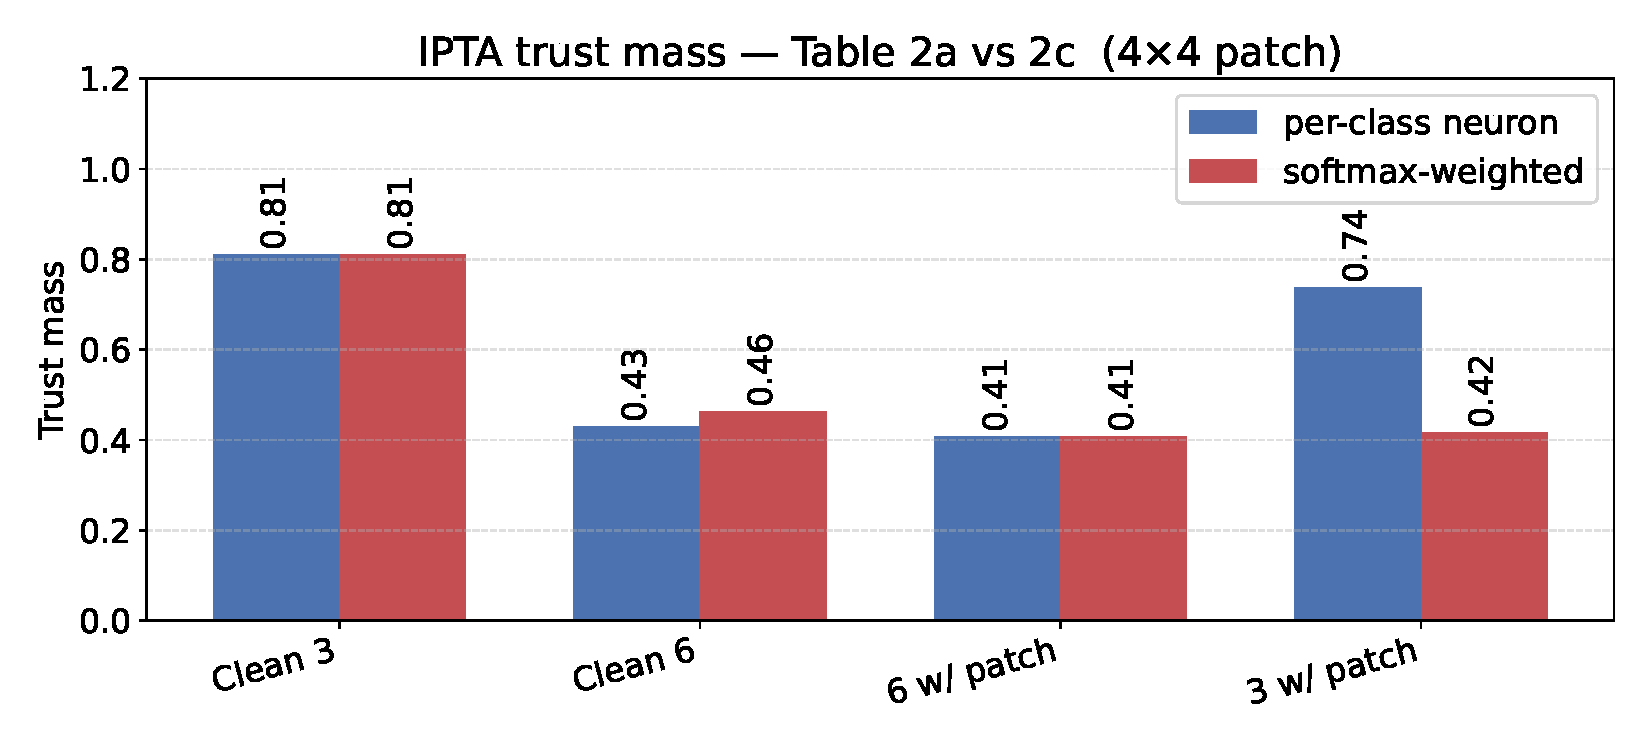
\includegraphics[width=0.8\linewidth]{latex/NN_Train_mnist_128_trust_trust_PathSize_4__ipta_trust_2a_vs_2c.pdf}
    \caption{IPTA trust mass comparison between per-class neuron and softmax-weighted aggregation ($\sum_i p_i t_i$) for the \ac{NN} trained on the poisoned dataset with patch size $4 \times 4$. The softmax-weighted aggregation weights each output neuron's trust mass by the model's predicted probability, producing a ranking that better reflects the reliability of the final decision rather than the inference path alone.}
    \label{fig:mnistpoisipta2}
\end{figure}



\section{Summary \& Conclusions}
\label{sec:patas-tp-conclusion}


This chapter presented \ac{PaTAS-TP}, a framework for propagating trust through
\acp{NN} in parallel with standard computation. The results are encouraging: trust
assessments converge alongside model training, respect theoretical symmetry and
invariance properties, and provide interpretable signals that complement accuracy
in all \DIFdelbegin \DIFdel{three }\DIFdelend \DIFaddbegin \DIFadd{four }\DIFaddend experimental settings. \DIFdelbegin \DIFdel{We consider this an initial contribution whose
viability is demonstrated on moderate-scale architectures; extending }\DIFdelend \DIFaddbegin \DIFadd{The comparative evaluation makes the framework's
value attributable rather than aggregate: input-space conformity carries violation
detection and composes with path trust into a per-sample score that fails safely,
the propagation itself contributes detection signal where input marginals are
silent, and the model-side trust yields per-class poisoning localization and a
test-data-free training-quality audit that no input-space or output-only baseline
expresses. The evaluation now covers residual convolutional networks at accuracies
defensible for their domains ($99.3\%$ MNIST, $88.7\%$ Fashion-MNIST, $84.5\%$
CIFAR-10) through the activity-weighted conv }\ac{IPTA}\DIFadd{; extending trust functions
to transformer components and normalization layers, and scaling }\DIFaddend the evaluation to
\DIFdelbegin \DIFdel{state-of-the-art models and }\DIFdelend \DIFaddbegin \DIFadd{top-tier }\DIFaddend training pipelines, \DIFdelbegin \DIFdel{such as transformer-based architectures or large-scale convolutional networks, is a natural and important direction }\DIFdelend \DIFaddbegin \DIFadd{remain natural directions }\DIFaddend for future work.

A known limitation of the current design is that it structurally penalizes deeper
architectures. Each additional layer introduces an extra discounting step that
attenuates the trust signal, so deeper networks inherit less trust from their
inputs regardless of their predictive performance. \DIFdelbegin \DIFdel{This is
a meaningful concern
given that modern architectures are typically deep. Adapting the framework to
compensate for depth, for instance by normalizing trust opinions with respect to path length or by using layer-wise trust scaling, is a direction for future work}\DIFdelend \DIFaddbegin \DIFadd{The depth-normalized
aggregation introduced in }\cref{sec:tp_arch_ovvw} \DIFadd{compensates for the geometric
component of this decay and makes trust values comparable across depths, and it is
used alongside the raw aggregate in the audit of Experiment~4; a fully
depth-invariant formulation of the propagation itself, rather than a corrected
readout, remains future work. Two further limitations surfaced by the comparative
evaluation deserve explicit mention. First, the trust functions combine opinions
independently of weight and activation magnitudes: trust deliberately tracks the
provenance and reliability of the quantities entering a computation rather than
their functional influence, so an input the network effectively ignores can still
contribute to the output opinion. Partial influence-aware steps exist, the
softmax-weighted aggregation of Experiment~3 and the activity-weighted conv
}\ac{IPTA}\DIFadd{, but fully magnitude-aware trust functions remain open. Second, the
conformity-based input opinions detect support violations, not support subsets;
the subset-direction }\ac{OOD} \DIFadd{failure is predicted by the a-priori diagnostics,
and fusing a covariance- or neighborhood-based detector into the input opinion
through the same quantification is the natural }\ac{SL} \DIFadd{remedy}\DIFaddend .

A second limitation concerns the directional preservation of evidence established
in \cref{thm:infvac} and its Remark. While theoretically sound, this property implies that \ac{PaTAS-TP} cannot generate a non-zero distrust mass at the output when the input carries no distrust, that is, when $d_x = 0$, even if the model parameters are highly unreliable. In other words, parameter unreliability manifests as increased uncertainty rather than explicit distrust in the output opinion. This is a genuine
restriction in safety-critical settings where a positive distrust signal would be
more actionable than a high uncertainty mass. Relaxing this constraint, for
instance by allowing parameter distrust to directly contribute a distrust component
to the output, is another avenue for future work.

Finally, the gradient-counting procedure used in \textsc{NodeTrust} fixes the
uncertainty component of the resulting binomial opinion based on the number of
input neurons, which may not be optimal in all cases. Adaptive quantification
schemes, as well as richer initialisation strategies for
$T_{n_i \mid \overline{y_\text{batch}}}$ beyond the vacuous opinion, are further
directions for improving the framework.





